\chapter{Measurement of NCQE
Interactions with the SK-Gd Upgrade}
\label{chp:ncqegd}


At energies close to the atmospheric peak, the NCQE interaction cross sections can be evaluated using T2K beam neutrinos. This chapter will present the status of the improved neutron tag from SK-Gd, its impact on the measurement of NCQE in T2K and the improvements to the SRN background measurement. The prompt and delayed signal of the NCQE interaction mimics that of the DSNB, due to the positron being the prompt signal for DSNB, while the prompt signal for NCQE is given by a gamma ray. Neutron capture constitutes the delayed signal for both SRN and NCQE interactions. With the recent addition of 0.026\% $\mathrm{Gd}_{2}\left(\mathrm{SO}_{4}\right)_{3} \cdot 8 \mathrm{H}_{2} \mathrm{O}$ to Super-Kamiokande, neutron detection has improved due to the  gamma cascade signal produced when neutrons are captured on gadolinium. 

There are multiple stages to this analysis, shown in Figure \ref{fig:analysis_flowchart}, where the ``neutron tagging'' stage occurs via two methods. Previously the NCQE neutron-tagging analyses used a method for neutron tagging which will be referred to as ``legacy NTag code'', but in 2020 the Super-K collaboration decided to proceed to use a new, more compact and streamlined version, which combines most of these stages into one piece of software. This will be referred to as``current NTag code'', and this is shown in Figure \ref{fig:analysis_flowchart} as well. The red arrows in Figure \ref{fig:analysis_flowchart} show the steps in the analysis prcoedure using the legacy NTag code which have been assimilated into the new NTag code.

\begin{figure}
    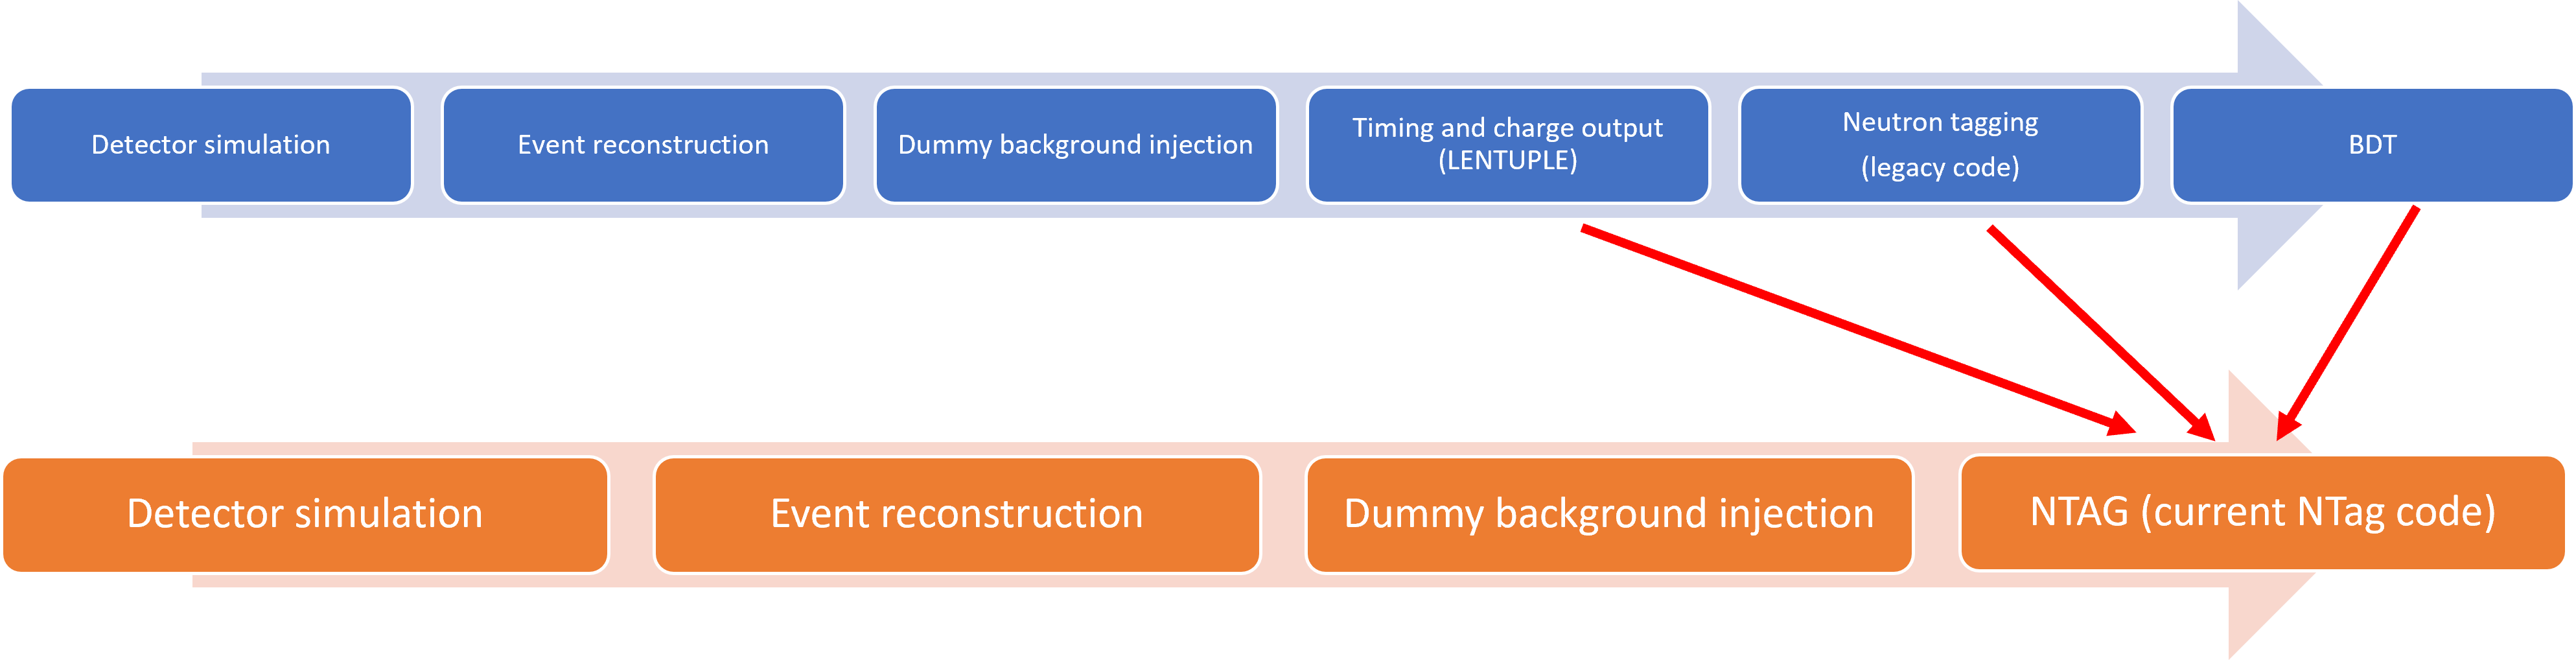
\includegraphics[width=\textwidth]{Figures/analysis_flowchart.png}
    \caption{Flowchart showing the stages in this analysis for both the analysis which used the legacy Ntag code (blue) and the current NTag code (orange).}
\label{fig:analysis_flowchart}
\end{figure}

A large portion of this analysis was to validate the results regarding the prompt event reconstruction and the neutron truth information between the legacy NTag and the new NTag - while the general neutron tagging algorithm was the same, the complete rearrangement of the structure of the NTag code required there to be checks regarding event reconstruction variable output and true neutron information variables such as the number of neutrons captured and the position in the detector the neutron captures occur at which will be shown later on in this Chapter. 

\section{Event Simulation}

This section discusses details about the event simulation, specifically the way neutrino interactions are simulated in order to produce the Monte Carlo. Table \ref{table:software} summarises all the software packages used in this analysis. 


\begin{table}
$$
\begin{array}{ll}
\hline \text { Name } & \text { Version } \\
\hline \text { Flux } & 13 \text { a tuning v4.0 } \\
\text { NEUT } & 5.3 .3 \\
\text { SKDETSIM-SKGd } & \text { ANNRI-Gd model } \\
\text { Geant } & 4.10.05.p01 \\
\text { T2KReWeight } & \text { v1r23 } \\
\text { GENIE } & \text { R2-12-10 } \\
\hline
\end{array}
$$
\caption{Software versions used in analysis from \cite{tn415_fiacob}.}
\label{table:software}
\end{table}

\subsection{Neutrino flux}

 As mentioned in Chapter 2, the T2K neutrino beam is generated by having a 30 GeV proton beam impinge on a graphite target, where the pions and kaons that result from this decay, producing in anti(neutrinos). Neutrino event rates measured at Super-Kamiokande are compared to Monte-Carlo predictions stemming from flux calculations. Prior to data from the NA61/SHINE experiment, the flux was predicted from hadron production models which were tuned to data which produced large systematic uncertainties. However, the NA61/SHINE experiment provides direct hadron production measurements for T2K and other long baseline experiments, and measures the yield of charged hadrons from a proton beam fired at a thin graphite target (2 cm long) and a T2K replica graphite target (90 cm long). From this experimental data, Monte Carlo simulations of the neutrino flux are predicted. In the beam MC, protons which have 30 GeV of kinetic energy are focused onto a graphite target and after the secondary particles are focused using the horn magnets, the neutrino tracks they decay into are ascertained at the near detectors and at Super-Kamiokande to produce the flux and energy spectra at both of these locations. The T2K neutrino beam flux version used in this analysis is 13a tuning v4.0 which uses the NA61/SHINE 2009 Replica-Target Data \cite{flux_ver}. Figure \ref{fig:energy_spectra} shows the energy spectra of each of the neutrino flavour components for the FHC (forward horn current) mode for the T2K Run 1-9 period. 
 
\begin{figure}
    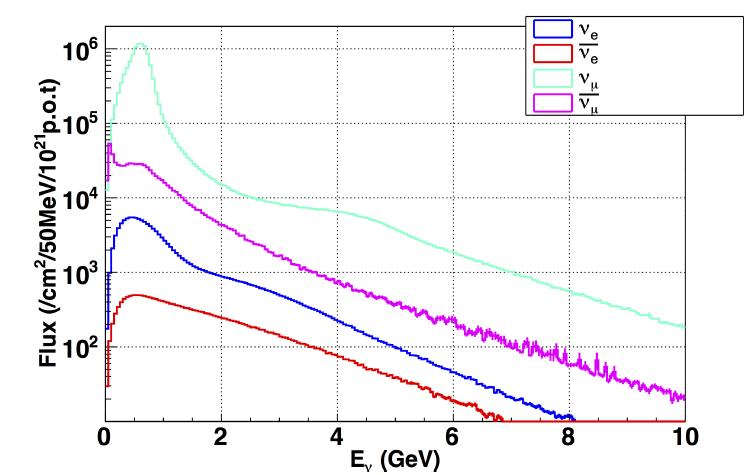
\includegraphics[width=0.8\textwidth]{Figures/energy_spectra.png}
    \caption{Energy spectra of the  $\left(\nu_{e}, \overline{\nu_{e}}, \nu_{\mu}, \overline{\nu_{\mu}}\right)$ flavour components for the FHC mode, T2K Run 1-9. }
\label{fig:energy_spectra}
\end{figure}
 
 
 The oscillation effect on the neutrino flux also needs to be considered after choosing which flux to use: the neutrino-oxygen NCQE cross section does not depend on flavour, and therefore neutrino oscillation affects would have no impact on a fully pure NCQE sample. However, there is a small fraction of charged current events which seep into the NCQE sample, and oscillation weights need to be applied to the charged current events in the sample. The entire Monte Carlo is reweighted as if it was fully comprised of muon and muon anti-neutrinos, due to the very small presence of electron neutrinos. Equation \ref{eq:flux_reweighting} shows the event weight applied to charge current events for the 2-flavour (electron neutrino and muon neutrino) scenario.

 \begin{equation}
 \begin{aligned}
 \text { weight }\left(E_\nu\right) & =P_{\nu_\mu \rightarrow \nu_\mu}\left(E_\nu\right)+P_{\nu_\mu \rightarrow \nu_e}\left(E_\nu\right) \times \underbrace{\frac{\sigma_{\nu_e C C}\left(E_\nu\right)}{\sigma_{\nu_\mu C C}\left(E_\nu\right)}}_{\approx 1} \\
 & \approx P_{\nu_\mu \rightarrow \nu_\mu}\left(E_\nu\right)+P_{\nu_\mu \rightarrow \nu_e}\left(E_\nu\right) \\
 & =1-\cos ^4 \theta_{13} \times \sin ^2 2 \theta_{23} \times \sin ^2\left(1.267 \frac{\Delta m_{32}^2\left[\mathrm{eV}^2\right] \cdot L[\mathrm{~km}]}{E_\nu[\mathrm{GeV}]}\right)
 \label{eq:flux_reweighting}
 \end{aligned}
\end{equation}

where the cross-section ratio term is simplified to 1 due to the kinematic difference between $e^{\pm}$ and $mu^{\pm}$ not being considered. Table \ref{table:osc_param} shows the oscillation parameters used in Equation \ref{table:osc_param} which are estimated with the reactor constraint taken from \cite{tn_osc_param}.

\begin{table}
\centering
\begin{tabular}{cc}
    \hline \text{Osc Parameter} & \text{Value} \\
    \hline $\sin ^2 \theta_{13}$ & $0.0211 \pm 0.0008$ \\
    $\sin ^2 \theta_{23}$ & $0.541_{-0.037}^{+0.027}$ \\
    $\left|\Delta m_{32}^2\right|$ & $2.469_{-0.071}^{+0.073} \times 10^{-3} \mathrm{eV}^2$ \\
    \hline
\end{tabular}
\caption{Oscillation parameters estimated with the reactor constraint.}
\label{table:osc_param}
\end{table}


\subsection{Primary interaction}

The interaction between the incoming neutrino event and an Oxygen nucleus, and the de-excitation of the nucleus is modelled by NEUT, which produces a vector of primary particles used for event simulation in SKDETSIM. Because these are primary particles, they do not take into consideration all the particles produced from the detector response, i.e. the secondary particles produced from the interactions within the medium of the detector, in our case, water doped with $\mathrm{Gd}_{2}\left(\mathrm{SO}_{4}\right)_{3} \cdot 8 \mathrm{H}_{2} \mathrm{O}$. The way NEUT treats the interaction between a nucleus and a neutrino for the case of a neutrino interaction with a ${ }^{16} \mathrm{O}$ isotope is shown in Figure \ref{fig:neutrinonuc}. 

\begin{figure}
    \centering
    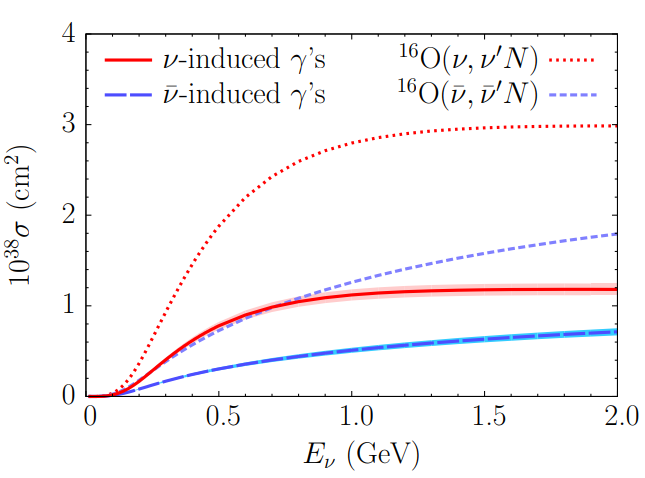
\includegraphics[width=0.7\textwidth]{Figures/neutrinonuc.png}
    \caption{Plot showing the NCQE cross section for ${ }^{16} \mathrm{O}$ as a function of incoming neutrino energy and the cross section of gamma ray production, taken from \cite{neutrino_nuc}.}
\label{fig:neutrinonuc}
\end{figure}
 

 NCQE interactions are modelled in NEUT using the Benhar Spectral Function (SF), while CCQE interactions (including 2p2h interactions) are modelled using the Relativistic Fermi-Gas (RFG) model \cite{benhar_electron-_2005}, \cite{rfg_model}. 2p2h interactions (2-particle-2-hole) involve a neutrino knocking nucleons out of a nucleus and creating two holes.


\begin{figure}
    \centering
    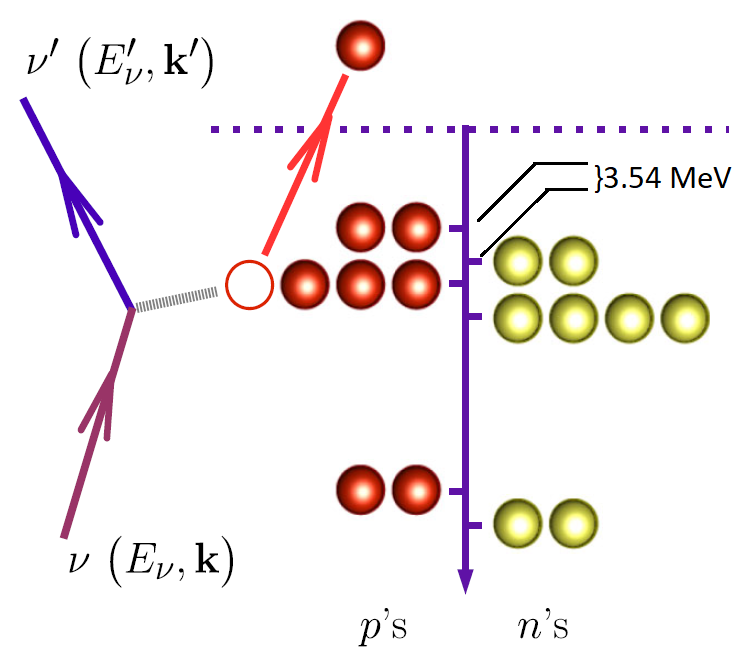
\includegraphics[width=0.7\textwidth]{Figures/ncqebenharspectral.png}
    \caption{Representation of NC neutrino scattering off ${ }^{16} \mathrm{O}$ with protons on the left hand side and neutrons on the right arranged according to the shell model. }
\label{fig:ncqebenharspectral}
\end{figure}

The lowest rung of nucleons in Figure \ref{fig:ncqebenharspectral} is the $s_{1/2}$, with $p_{3/2}$ above this level and $p_{1/2}$ above that. The protons in these rungs have removal energies of 42 MeV, 18.4 MeV and 12.1 MeV respectively, and due to neutron levels being more tightly bound, these have an extra removal of 3.24 MeV compared to their proton counterparts. The shell model is imperfect due to how it allocates the probablity of ${ }^{16} \mathrm{O}$ transitioning to the possible nucleon states. In the shell model, probabilities are allocated by counting the number of nucleons in each energy level and assigning probailities according to how many there are. In Figure \ref{fig:ncqebenharspectral} it can be seen that the $p_{3/2}$ state has double the number of nucleons compared to the $s_{1/2}$ model and therefore double the probability of transition is assigned for the $p_{3/2}$ state, and the probability of transitioning to any other state is assigned to be 0, because in the shell model they don't even exist. The Benhar Spectral Function model however is complex and is tuned using electron-nucleus scattering data. The model used in this analysis is a modified version of the Benhar Spectral Function model, where the case of other transition states is dealt with by merging the ``others'' state into the $s_{1/2}$ state. Table \ref{table:transitionprob} gives the probabilities of transition to different states for different models. 

\begin{table}
$$
\begin{array}{ccccc}
\hline & \left(\mathrm{s}_{1 / 2}\right)^{-1} & \left(\mathrm{p}_{3 / 2}\right)^{-1} & \left(\mathrm{p}_{1 / 2}\right)^{-1} & \text { others } \\
\hline \text { Shell model } & 0.25 & 0.5 & 0.25 & 0 \\
\text { Spectral Function } & 0.1055 & 0.3515 & 0.158 & 0.385 \\
\text { This analysis } & 0.4905 & 0.3515 & 0.158 & 0 \\
\hline
\end{array}
$$
\caption{Transition probabilities for different models and states}
\label{table:transitionprob}
\end{table}

\subsection{Detector response and interactions in the detector medium}

Prior analyses to this used SKDETSIM (Super-Kamiokande Detector Simulator) to simulate the trajectories of particles through the water in Super-Kamiokande and output detector response MC. This analysis uses SKDETSIM-SKGd to propogate the particles, due to the requirement of needing gadolinium sulphate present in the simulation. Unlike SKDETSIM, SKDETSIM-SKGd has a GEANT4 function implemented for neutron capture on gadolinium isotopes and its subsequent interactions. The particular isotopes of gadolinium used in the simulation are ${ }^{155} \mathrm{Gd}$ and ${ }^{157} \mathrm{Gd}$ due to their excellent thermal neutron capture cross sections. Table \ref{table:gdtable} shows the relative abundance of various gadolinium isotopes inside natural gadolinium and their associated thermal neutron capture cross sections.

\begin{table}
$$
\begin{array}{rcc}
\hline \text { Isotope } & \text { Abundance }[\%] & \text { Cross-section[b] } \\
\hline{ }^{152} \mathrm{Gd} & 0.200 & 735 \\
{ }^{154} \mathrm{Gd} & 2.18 & 85 \\
{ }^{155} \mathbf{Gd} & \mathbf{1 4 . 8 0} & \mathbf{6 0 9 0 0} \\
{ }^{156} \mathrm{Gd} & 20.47 & 1.8 \\
{ }^{157} \mathbf{Gd} & \mathbf{1 5 . 6 5} & \mathbf{2 5 4 0 0 0} \\
{ }^{158} \mathrm{Gd} & 24.84 & 2.2 \\
{ }^{160} \mathrm{Gd} & 21.86 & 1.4 \\
\hline
\end{array}
$$
\caption{Abundance and thermal neutron capture cross section of various isotopes of Gadolinium}
\label{table:gdtable}
\end{table}

As can be seen in Table \ref{table:gdtable}, not only are ${ }^{155} \mathrm{Gd}$ and ${ }^{157} \mathrm{Gd}$ have extremely high neutron capture cross sections compared to the other isotopes. Equation \ref{eq:gdisotopecaptureeq} shows the neutron capture on both of these isotopes, and the energy of the subsequent gamma rays.

\begin{equation}
\begin{split}
 {n}+{ }^{155} \mathrm{Gd} \rightarrow{ }^{156} \mathrm{Gd}^{*} \rightarrow{ }^{156} \mathrm{Gd}+\gamma  (8.536 MeV)\\
 {n}+{ }^{157} \mathrm{Gd} \rightarrow{ }^{158} \mathrm{Gd}^{*} \rightarrow{ }^{158} \mathrm{Gd}+\gamma  (7.937 MeV)
\end{split}
\label{eq:gdisotopecaptureeq}    
\end{equation}




It is important to therefore model the gamma ray emission spectra from both of these isotopes. The model used by SKDETSIM-SKGd is the ANNRI-Gd model, \cite{annri_gd_energy}, \cite{tanaka_gamma_2020}. This uses gamma energy spectrum data from the germanium spectrometer at the ANNRI (Accurate Neutron Nucleus Reaction Measurement Instrument) experiment. This experiment uses the incoming pulsed neutron beam from the Japan Spallation Neutron Source (JSNS) at the Material and Life Science Experimental Facility (MLF) of J-PARC. After a 300 kW beam of protons from the JSNS facility hits a target of mercury and produces neutrons, this neutron beam hits an enriched ${ }^{155} \mathrm{Gd}$ target or a ${ }^{nat} \mathrm{Gd}$ film. The ANNRI spectrometer is placed 21.5 m away from the neutron beam source, with two cluster detectors on either side of the neutron capture target material, which is 13.4 cm away from each cluster detector. Surrounding the target, there are also 8 co-axial germanium detectors. The schematic for the ANNRI-Gd experiment is shown in Figure \ref{fig:annrigd}.

\begin{figure}

        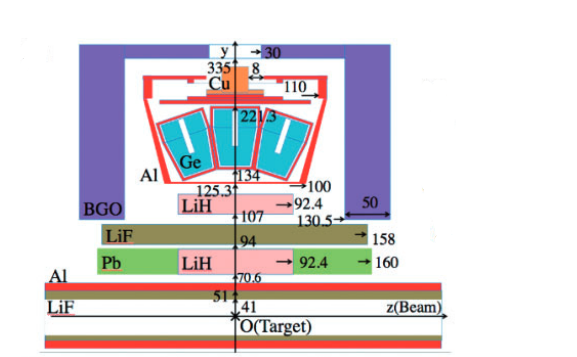
\includegraphics[width=\textwidth]{Figures/annrigd.png}
        \caption{Schematic of the ANNRI Ge spectrometer (dimensions in mm). The beam pipe along with one of the Ge cluster detectors (light blue) is shown. The shaded purple area are the anti-coincidence shields made of bismuth-germanium-oxide (BGO) crystals \cite{annri_gd_energy}.}
        \label{fig:annrigd}
    
\end{figure}

Figure \ref{fig:annrigdenergyspectra} shows the energy spectra for different multiplicity values (left) and hit values (right) from one of the germanium crystals in the ANNRI spectrometer. 

\begin{figure}
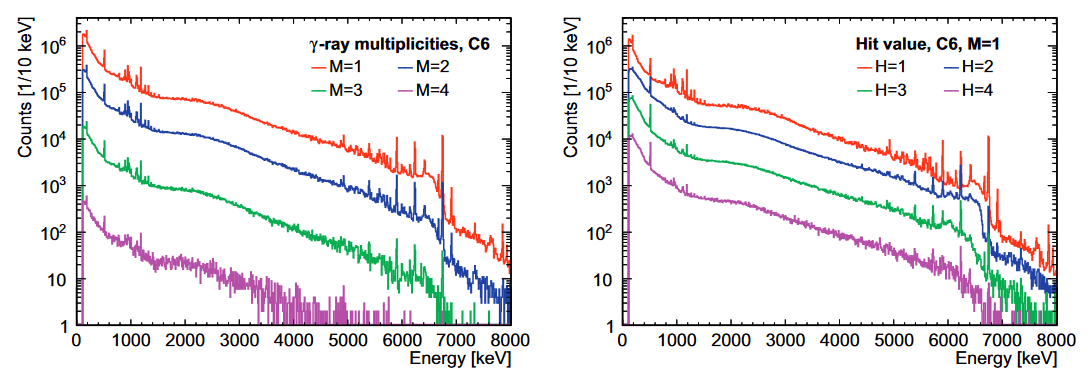
\includegraphics[width=\textwidth]{Figures/annrigdenergyspectra.png}
\caption{Energy spectra for thermal neutron capture on ${ }^{157} \mathrm{Gd}$ energy spectra for different multiplicity values (left) and hit values (right) from one of the germanium crystals in the ANNRI spectrometer. Taken from \cite{annri_gd_energy}.}
\label{fig:annrigdenergyspectra}
\end{figure}

One of the key differences between the default Geant4 model for thermal neutron capture on Gadolinium and the ANNRI-Gd model is how it conserves energy: the photon evaporation model conserves only the final sum of energy for the captured event, but performs poorly when modelling the gamma-ray energy on an individual event by event basis. One way the ANNRI-Gd model combats this is by seperately describing the continuous and discrete peaks in Figure \ref{fig:annrigdenergyspectra}, where the discrete peaks are shown as spikes below 1500 keV and above 4500 keV. These come from the different ways in which gadolinium de-excites after thermal neutron capture. The continuous spectrum in the plots in Figure \ref{fig:annrigdenergyspectra} show the de-excitation of ${ }^{158} \mathrm{Gd}^{*}$ in multiple steps, producing multiple low energy gamma rays, which accounts for about 93\% of the spectrum. The discrete spikes in the spectra come from a two-step cascade, which produces a high energy gamma ray instead, accounting for the remaining 7\% of the spectrum.
Figure \ref{fig:continousdiscrete} shows the continuous and discrete components of the ANNRI-Gd MC, along with data from the experiment. Figure \ref{fig:annrigdmodelcompare} shows ratio plot of data and MC for the GLG4sim model, the default Geant4 photon evaporation model and the ANNRI-Gd model: here it is clear the ANNRI-Gd model fits the data better than the other two models, especially at energies above 3500 keV. The energy from the neutron capture on Gadolinium de-excitation is released in the form of multiple gamma rays, and liquid scintillator detectors would only have to look for the deposition of the energy from these gamma rays, whereas a water Cherenkov detector such as Super-Kamiokande can only detect part of this deposition due to the Cherenkov threshold energy. As a result, understanding the gamma ray multiplcities and their energies in the range 0.8 MeV to 8 MeV is important in order to predict the efficiency of neutron tagging within Monte Carlo simulation.


\begin{figure}
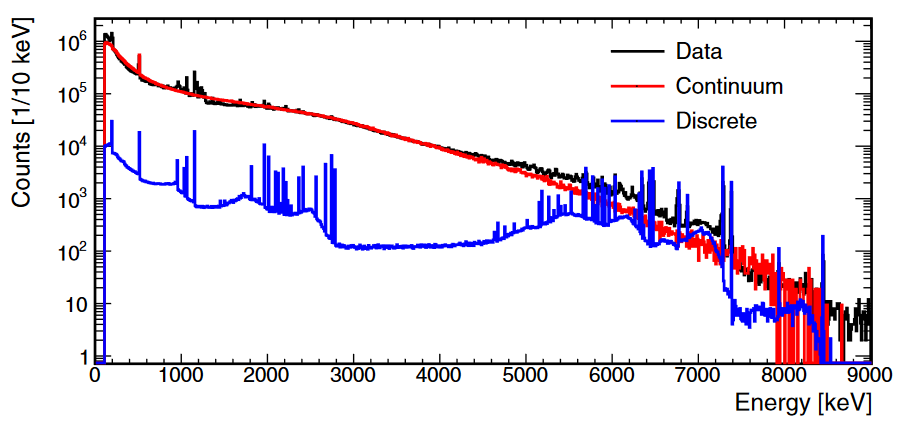
\includegraphics[width=\textwidth]{Figures/continousdiscrete.png}
\caption{Energy spectra for the ANNRI-Gd model broken down into its continous and discrete components along with data from the ANNRI-Gd experiment \cite{annri_gd_energy}.}
\label{fig:continousdiscrete}
\end{figure}

\begin{figure}
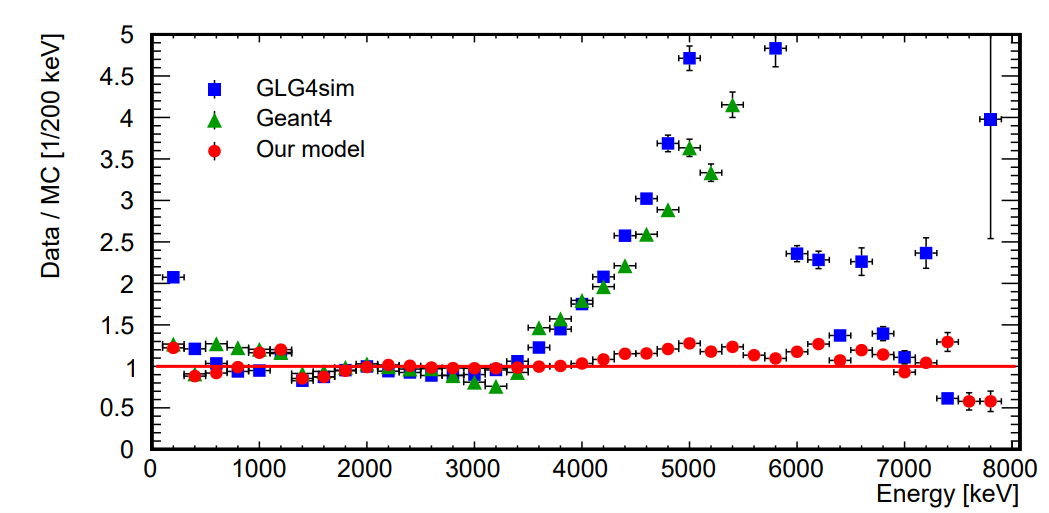
\includegraphics[width=\textwidth]{Figures/annrigdmodelcompare.png}
\caption{Comparison between neutron capture MC models and ANNRI-Gd data, with the ratio of data and MC on the y-axis, the GLG4sim model in blue, Geant4 default model in green and the ANNRI-Gd model in red \cite{annri_gd_energy}.}
\label{fig:annrigdmodelcompare}
\end{figure}


\section{Event Reconstruction}
\subsection{Bonsai output reconstruction quantities}

Due to this analysis looking specifically at the low energy region, a fitter (LOWFIT) specific to low energies (below 100 MeV) is used to reconstruct events. Both MC and data neutrino events undergo a reconstruction phase, where the low-energy fitter BONSAI is applied to the event, as discussed in Chapter 2. The reconstruction is carried out using timing and PMT position information, however charge information is omitted - this is because of only a couple photoelectrons being produced by each PMT, so it makes sense to count the number of hit PMTs instead. The output of BONSAI gives information which will be used in the reduction phase of the data and allow for the selection of the NCQE sample. The following quantities comprise the BONSAI output, the first two being helpful spectator variables and the latter five constituting parameters which are used in the reduction phase of the analysis, from which the neutrino NCQE sample is determined.\\


\noindent
\underline{1. Neutrino vertex position}\\
\noindent 
The reconstructed location of the neutrino interaction event.

\noindent
\underline{2. Neutrino vertex direction}\\
\noindent
This vector points towards the direction which is an average over all the Cherenkov cone axes which are produced, due to there being multiple leptons induced in the interaction.


\noindent
\underline{3. Reconstructed energy}\\
\noindent 
In line with the standard SK low energy analysis definition, this energy is simply the reconstructed kinetic energy of the electrons. 


\noindent
\underline{4. Dwall}\\
\noindent 
This variable gives the minimum distance of the neutrino vertex position from the closest wall of the Super-Kamiokande detector.

\noindent
\underline{5. Effwall}\\
\noindent 
This variable gives the distance between the neutrino vertex position and the closest wall, but moving back from the vertex position along the neutrino vertex direction vector.

\noindent
\underline{6. Vertex direction and goodness coefficient}\\
\noindent 
The coefficient $ovaQ$ (defined in Equation \ref{eq:ovaq}) describes the quality of the vertex reconstruction. It consists of two parameters $g^2_{vtx}$ and $g^2_{dir}$ where the former describes the goodness of the vertex which is based on PMT hit timings, and increases the sharper an event is in time. The latter is the directional goodness and measures the azimuthal uniformity in the ring pattern produced by the Cherenkov cone, which decreases the more uniform an event is in space. As a result of this, $ovaQ$ increases the more uniform and sharp in time an event is.

\begin{equation}
    \text { ova } Q=g_{\text {vtx }}^{2}-g_{\text {dir }}^{2}
    \label{eq:ovaq}
\end{equation}

$g_{vtx}$ is calculated using a fit of the PMT timing distribution and using the hit times of the PMT it is defined as in Equation \ref{eq:vertex_goodness}.

\begin{equation}
g_{\mathrm{vtx}}=\frac{\sum_{i} w_{i} \mathrm{e}^{-\frac{1}{2}(\frac{\Delta t_{i}}{\sigma})^{2}}}{\sum_{i} w_{i}} \text { with } w_{i}=-\frac{1}{2}(\frac{\Delta t_{i}}{\omega})^{2}
\label{eq:vertex_goodness}
\end{equation}

Here $\sum_{i} w_{i}$ is the weight given to the i-th hit PMT for the reduction of dark noise, where $\omega$ has a value of 60ns. $\sigma$ has a value of 5ns which is used to test the goodness, and as a result, a sharp timing distribution produces a large vertex goodness. $g_{dir}$ is calculated by looking at how spatially uniform the PMT hits are in the azimuthal angle around the reconstructed neutrino vertex direction. The hits are ordered from 0 to 2$\pi$ and compared to a uniform distribution of angles. Equation \ref{direction_goodness} shows how the minimum difference between the uniform distribution and the data is subtracted from the maximum difference and normalized to produce $g_{dir}$ .

\begin{equation}
    \mathrm{g}_{\mathrm{dir}}=\frac{\max _{i}\{\angle_{\mathrm{uni}}(i)-\angle_{\mathrm{data}}(i)\}-\min _{i}\{\angle_{\mathrm{uni}}(i)-\angle_{\mathrm{data}}(i)\}}{2 \pi}
\label{direction_goodness}
\end{equation}

where $\angle_{\mathrm{data}}(i)$ is the azimuthal angle of i-th hit real PMT included in the number of hits in 50ns. $\angle_{\mathrm{uni}}(i)=2 \pi i / N_{50}$ is the azimuthal angle of the i-th virtual PMT hit, but only when uniform distribution of the hits is assumed. As the uniformity of the hit pattern increases, the goodness decreases. 
 


\noindent
\underline{7. Cherenkov angle $\theta_{C}$}\\
\noindent

In order to estimate the Cherenkov opening angle, all the possible combinations of PMT hits of three hit PMTs in a 15 nanosecond timing window are binned. A histogram is produced of these binned angles and divided into 100 bins, and by looking at the seven neighbouring bins with the largest number of entries, peaks in the histogram are located. The middle of the seven bins is chosen to be the Cherenkov angle of the event. Figure \ref{fig:cherenkov_hit_triplet} shows the vertex of the prompt event and three PMT hit vectors which produce the Cherenkov opening angle. 

\begin{figure}
    \centering
    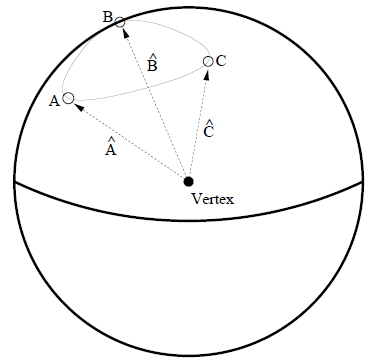
\includegraphics[width=0.5\textwidth]{Figures/cherenkov_hit_triplet.png}
    \caption{Schematic of the prompt event vertex and a triplet of independent PMT hits whch make up the Cherenkov angle, taken from \cite{malek_thesis}.}
    \label{fig:cherenkov_hit_triplet}

\end{figure}


 For relativistic electrons in water, the value of the Cherenkov opening angle is $\approx 42\degree$, due to the relation: 

 \begin{equation}
\cos \theta_{\mathrm{Cherenkov}}=\frac{1}{n\beta}
\label{cherenkov_angle}
\end{equation}
 
where $\beta = v/c \approx 1$ and $n$ is the refractive index of water, 1.33. However due to other particles in the simulation, such as protons or muons, the Cherenkov cone is expected to be narrower, or if multiple leptons are present, the Cherenkov cones will be less distinct and more spread out, leading to deviations from the 42$\degree$ value. 

\subsection{Comparison of BONSAI reconstruction output variables between SKDETSIM versions}

The BONSAI reconstruction output variables were compared between three versions of SKDETSIM, the version used in the previous NCQE neutron capture on hydrogen only analysis, with no neutron capture on Gd implemented (black), the SKDETSIM-SKGd photon-evaporation model mentioned in the previous section (red), and the SKDETSIM SK-Gd ANNRI-Gd model (green). Figure \ref{fig:erec_compare} to Figure \ref{fig:thetaC_compare} shows the comparison of these models for the output BONSAI variables $E_{rec}$, dwall, effwall, ovaQ, and $\theta_C$, where the y-axis shows the number of events.

\begin{figure}
    \centering
    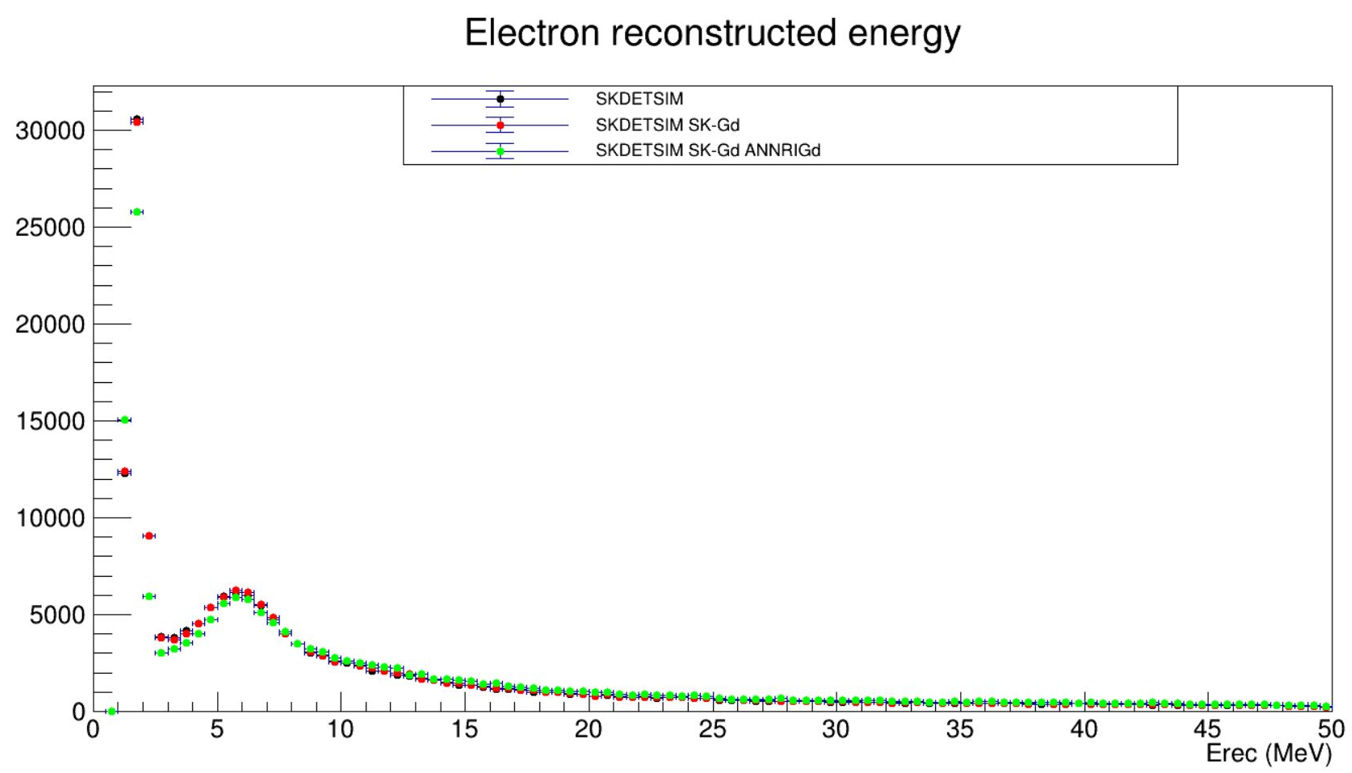
\includegraphics[width=0.8\textwidth]{Figures/erec_compare.png}
    \caption{Comparisons of prompt event electron reconstructed energy between versions of SKDETSIM}
    \label{fig:erec_compare}

\end{figure}

\begin{figure}
    \centering
    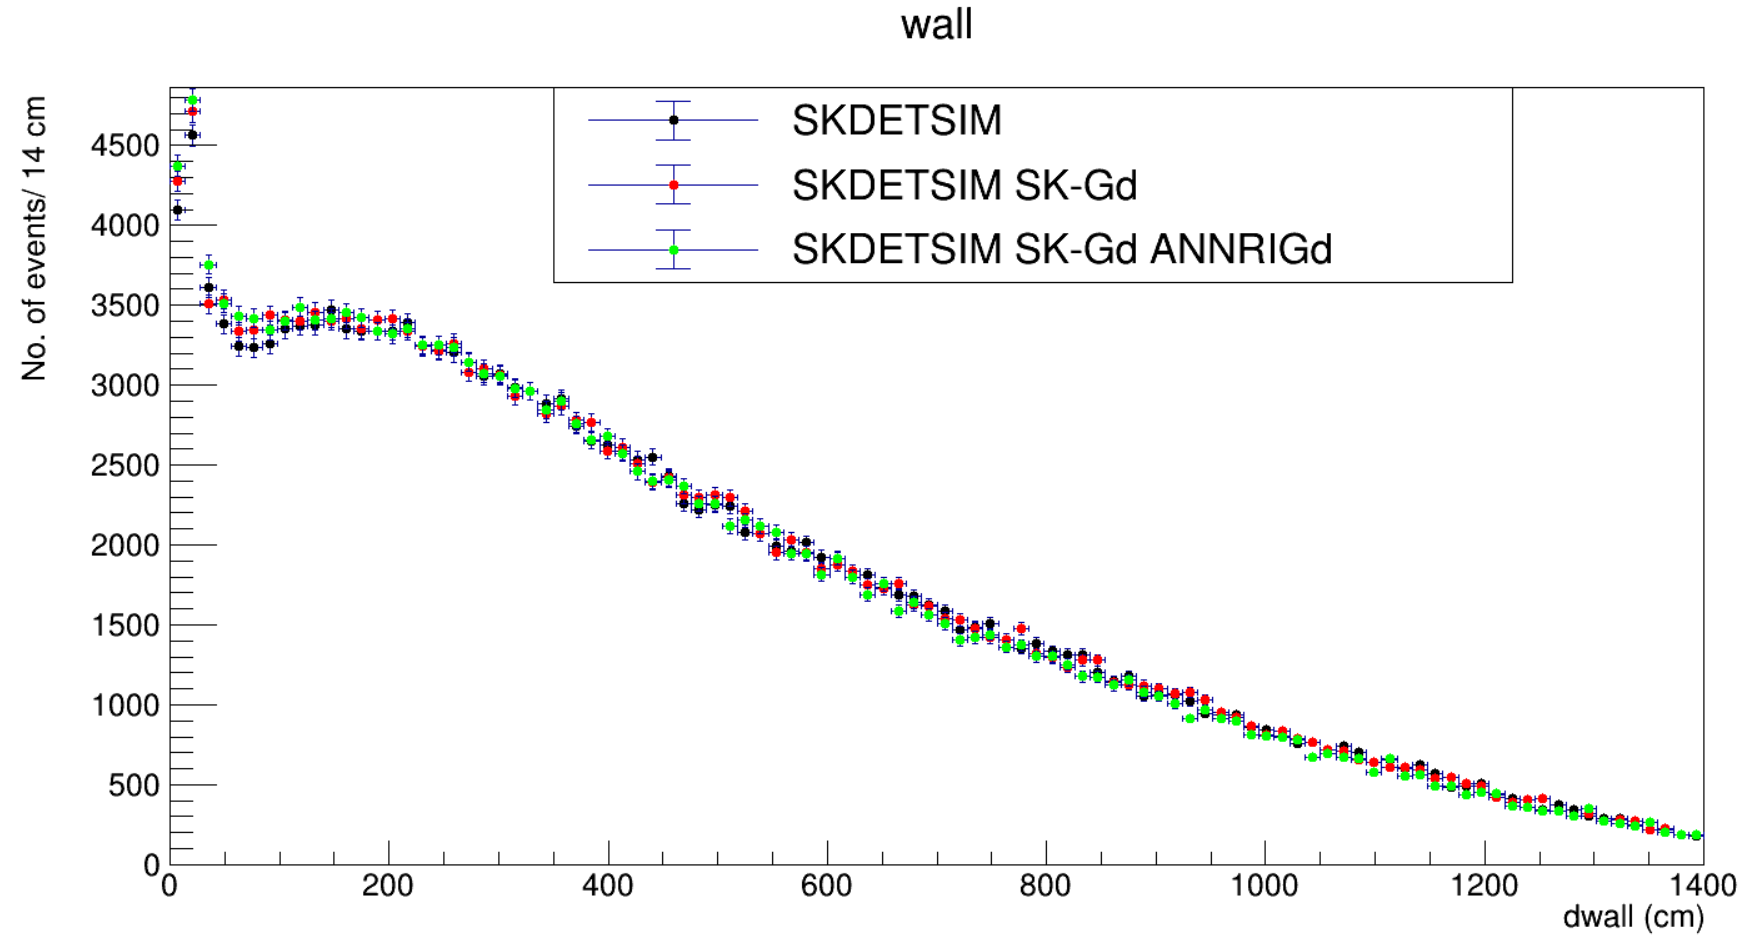
\includegraphics[width=0.8\textwidth]{Figures/dwall_compare.png}
    \caption{Comparisons of dwall for the prompt event between versions of SKDETSIM}
    \label{fig:dwall_compare}

\end{figure}

\begin{figure}
    \centering
    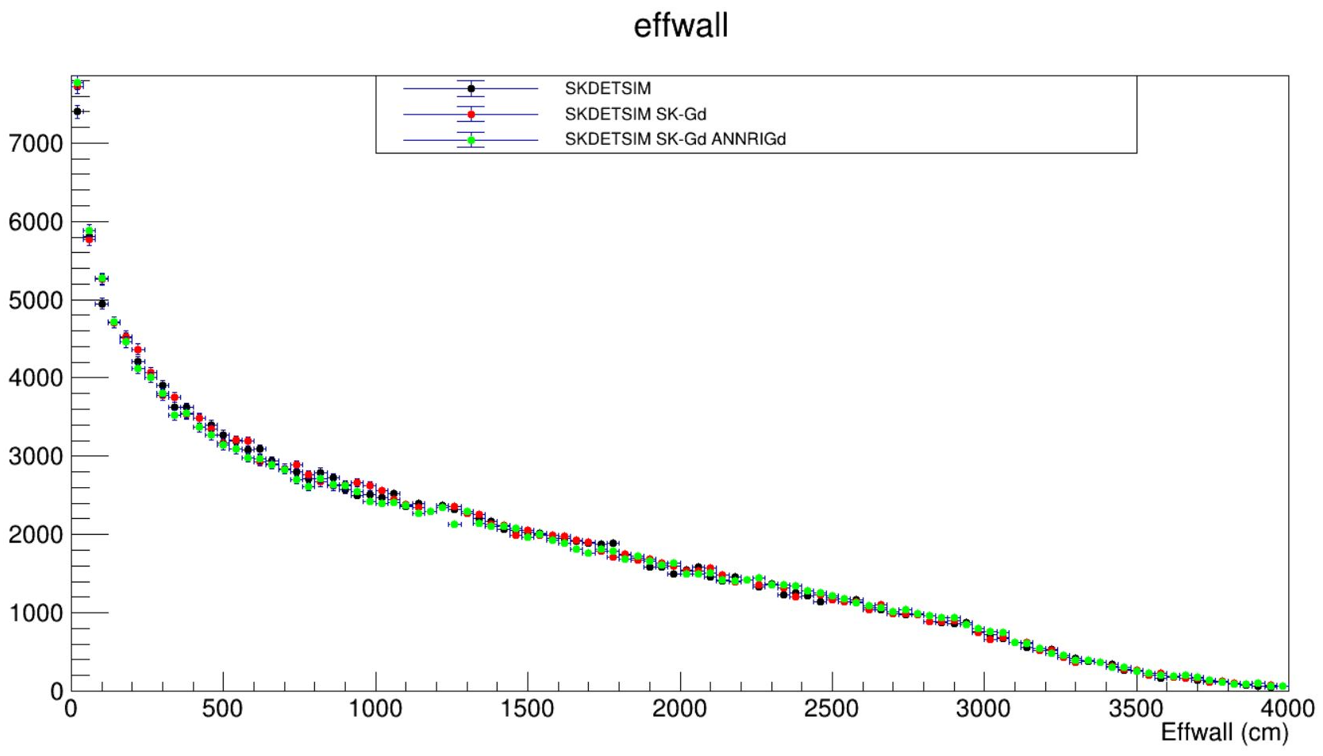
\includegraphics[width=0.7\textwidth]{Figures/effwall_compare.png}
    \caption{Comparisons of effwall for the prompt event between versions of SKDETSIM}
    \label{fig:effwall_compare}

\end{figure}

\begin{figure}
    \centering
    \includegraphics[width=0.7\textwidth]{Figures/ovaQ_compare.png}
    \caption{Comparisons of ovaQ for the prompt event between versions of SKDETSIM }
    \label{fig:ovaQ_compare}

\end{figure}

\begin{figure}
    \centering
    \includegraphics[width=0.7\textwidth]{Figures/thetaC_compare.png}
    \caption{Comparisons of Cherenkov angle for the prompt event between versions of SKDETSIM}
    \label{fig:thetaC_compare}

\end{figure}


To ensure correct implementation of the ANNRI-Gd model, ensuring the BONSAI output variables were similar between these SKDETSIM versions was important as the Gadolinium model should only effect the neutron capture in the simulation, not the output from event reconstruction of the neutrino interaction vertex. As can be seen in the SKDETSIM/SKDETSIM-SKGd BONSAI reconstruction variable comparison plots, this holds true for $E_{rec}$, dwall, effwall and $\theta_C$, but not for the vertex and goodness coefficient ovaQ, where the ANNRI-Gd model differs for ovaQ between -0.05 and 0.15 compared to the SKDETSIM and SKDETSIM photon-evaporation model. To investigate this difference further, distributions of the vertex goodness and the directional goodness which make up ovaQ (according to Equation \ref{eq:ovaq}) were also checked, shown in Figure \ref{fig:ovaQ_compare}.



\begin{figure}
    \centering
    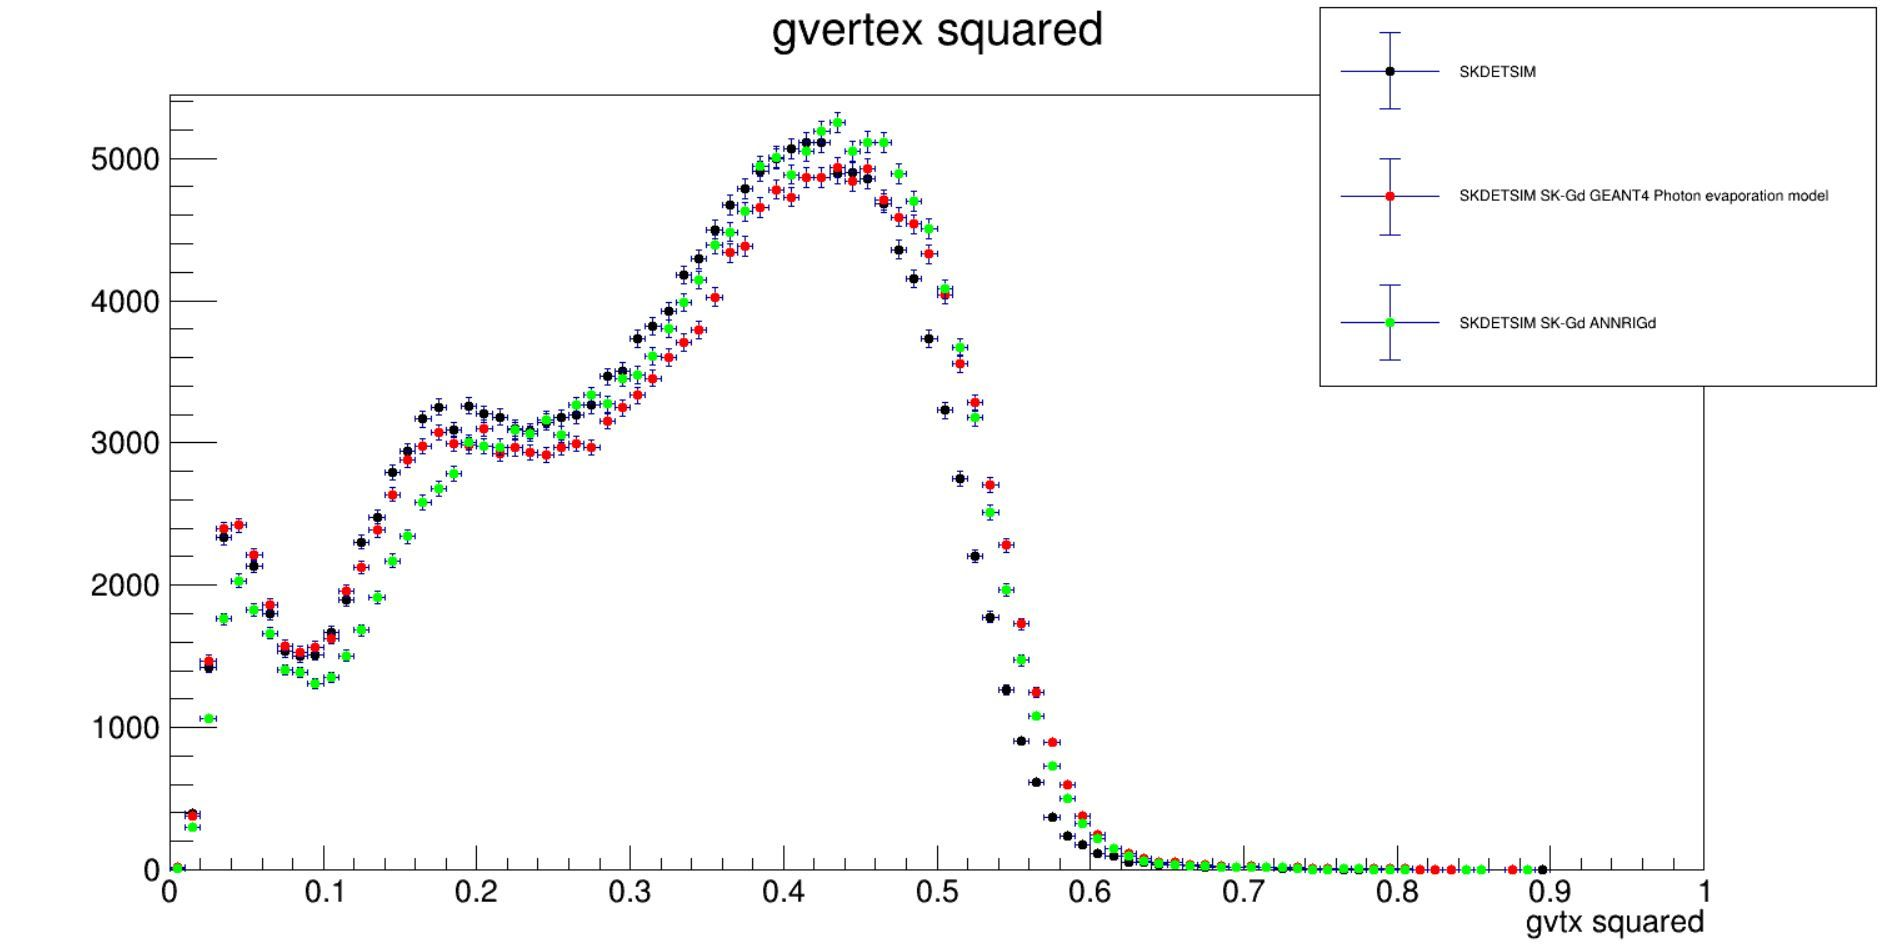
\includegraphics[width=0.8\textwidth]{Figures/gvtx_squared.PNG}
    \caption{Comparisons of vertex goodness for the prompt event between versions of SKDETSIM}
    \label{fig:gvtx_squared}

\end{figure}

\begin{figure}
    \centering
    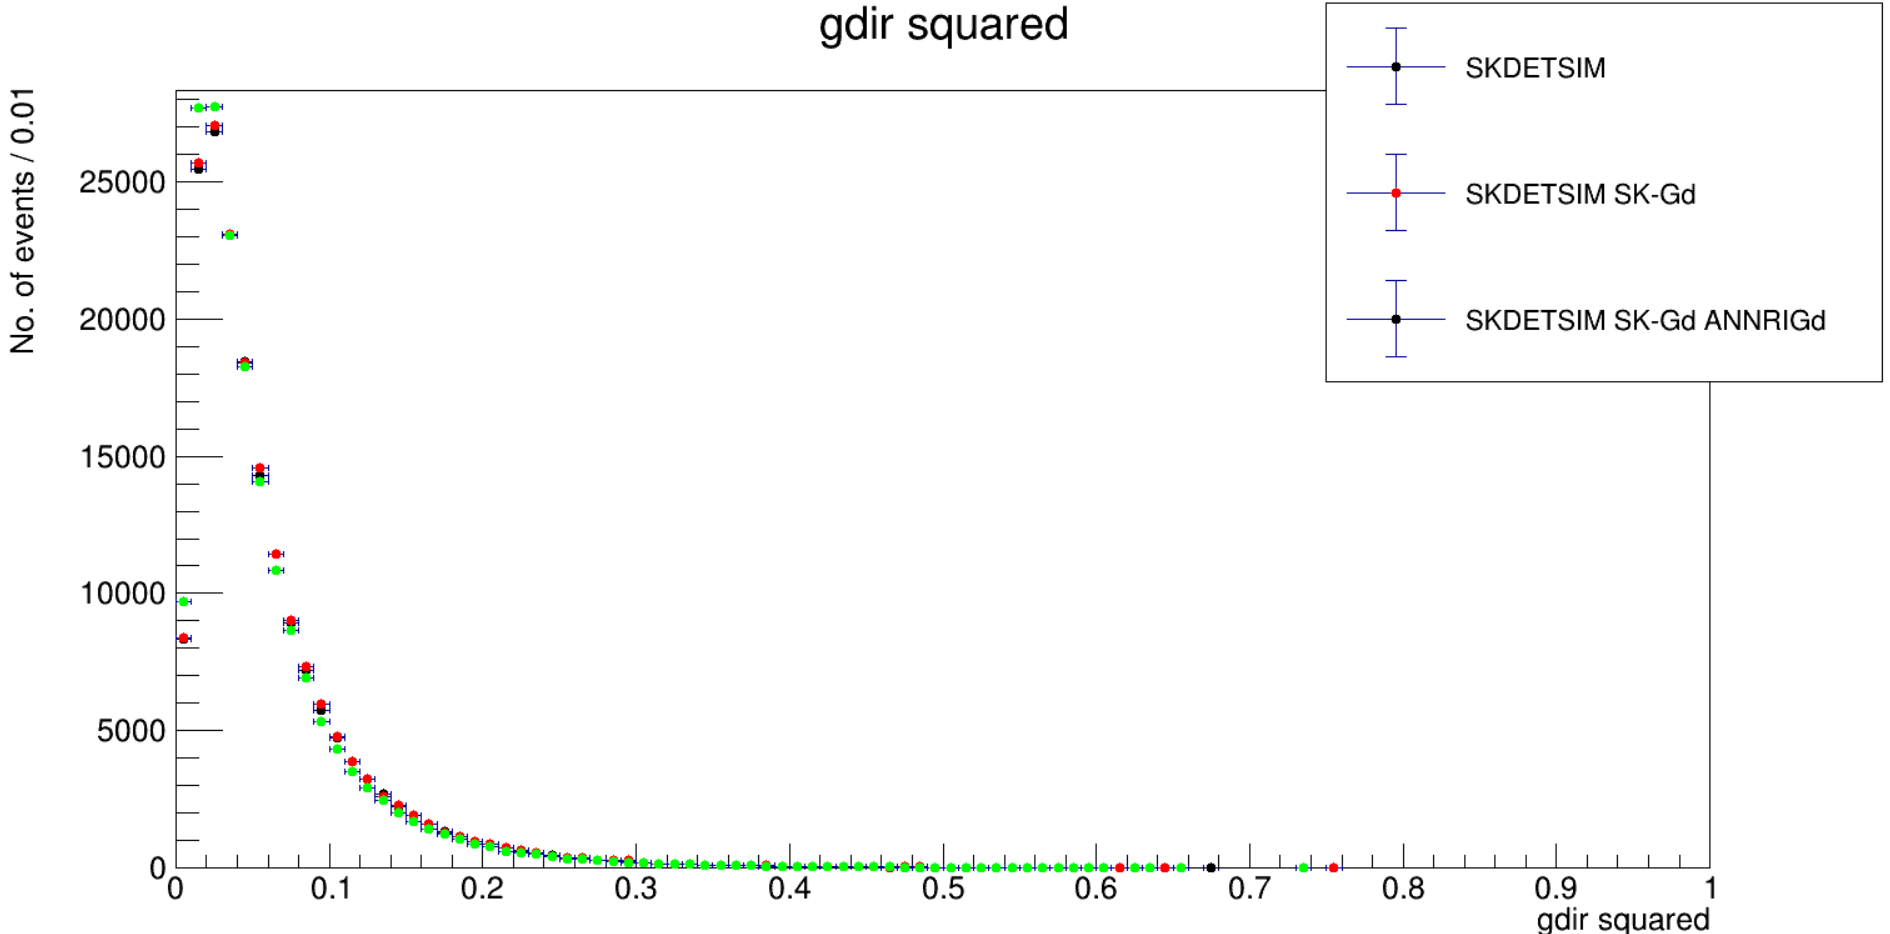
\includegraphics[width=0.8\textwidth]{Figures/gdir_squared.PNG}
    \caption{Comparisons of directional goodness for the prompt event between versions of SKDETSIM}
    \label{fig:gdir_squared}

\end{figure}

The vertex goodness (gvtx) and directional goodness (gdir) squared comparisons are shown in Figures \ref{fig:gvtx_squared} and \ref{fig:gdir_squared} respectively. Figure \ref{fig:gvtx_squared} shows a slight discrepancy between the SKDETSIM versions, but not enough to warrant further investigation. In addition to checking the previous BONSAI reduction phase quantities, the distance between the true neutrino vertex from the simulation and the neutrino vertex from the BONSAI reconstruction was also checked for the different SKDETSIM versions, shown in Figure \ref{fig:vertex_resolution}. Table \ref{table:vertex_resolution} shows the value of this distribution which encompasses 1-sigma (68\%) of the number of events: this value was very similar for all SKDETSIM versions.
\begin{figure}

    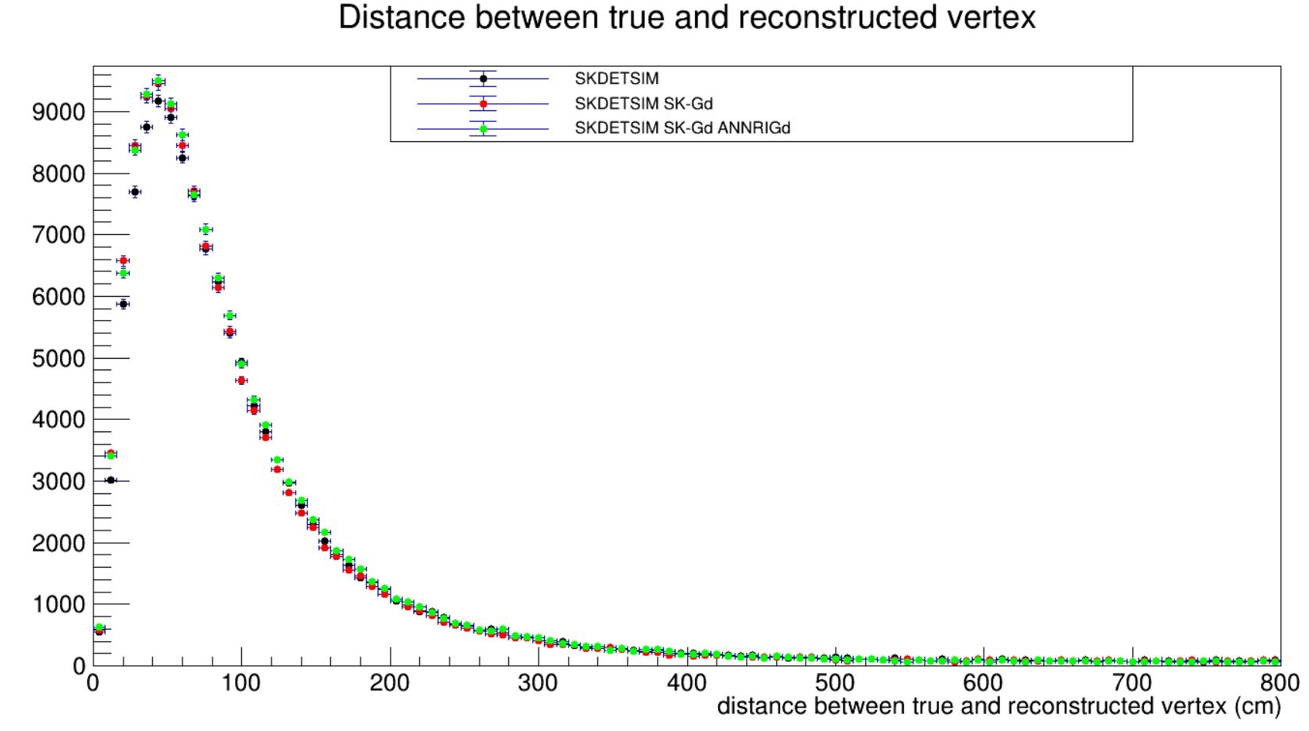
\includegraphics[width=0.8\textwidth]{Figures/vertex_resolution.png}
    \caption{Distance between true and reconstructed neutrino vertex for different SKDETSIM versions}
    \label{fig:vertex_resolution}

\end{figure}

\begin{table}
    $$
    \begin{array}{rcc}
    \hline \text { SKDETSIM version } & \text{Value (cm)} \\
    \text{SKDETSIM-V} & 113.2\\
    \text{SKDETSIM-SKGd (Photon evaporation model)} & 109.4 \\
    \text{SKDETSIM-SKGd (ANNRI-Gd model)} & 111.9 \\
    \hline
    \end{array}
    $$
\caption{Value of the true neutrino vertex - reconstructed neutrino vertex distribution which encompasses 1-sigma (68\%) of the number of events.}
\label{table:vertex_resolution}
\end{table}

\subsubsection{Comparisons of event reconstruction output between NTag versions}
To ensure that the NCQE event selection and neutron tagging could be carried out using the new NTag code, comparisons of the output BONSAI reconstruction variables between the two versions were made to ensure the validity of the reconstruction output. Figures \ref{fig:energy_recon_compare}, \ref{fig:dwall_recon_compare}, \ref{fig:effwall_recon_compare}, \ref{fig:angle_recon_compare} and \ref{fig:ovaq_recon_compare}  shows the reconstructed energy, dwall, effwall, Cherenkov angle and ovaQ parameters, with the legacy NTag output in black and the new NTag output in red. 


\begin{figure}
        \centering
        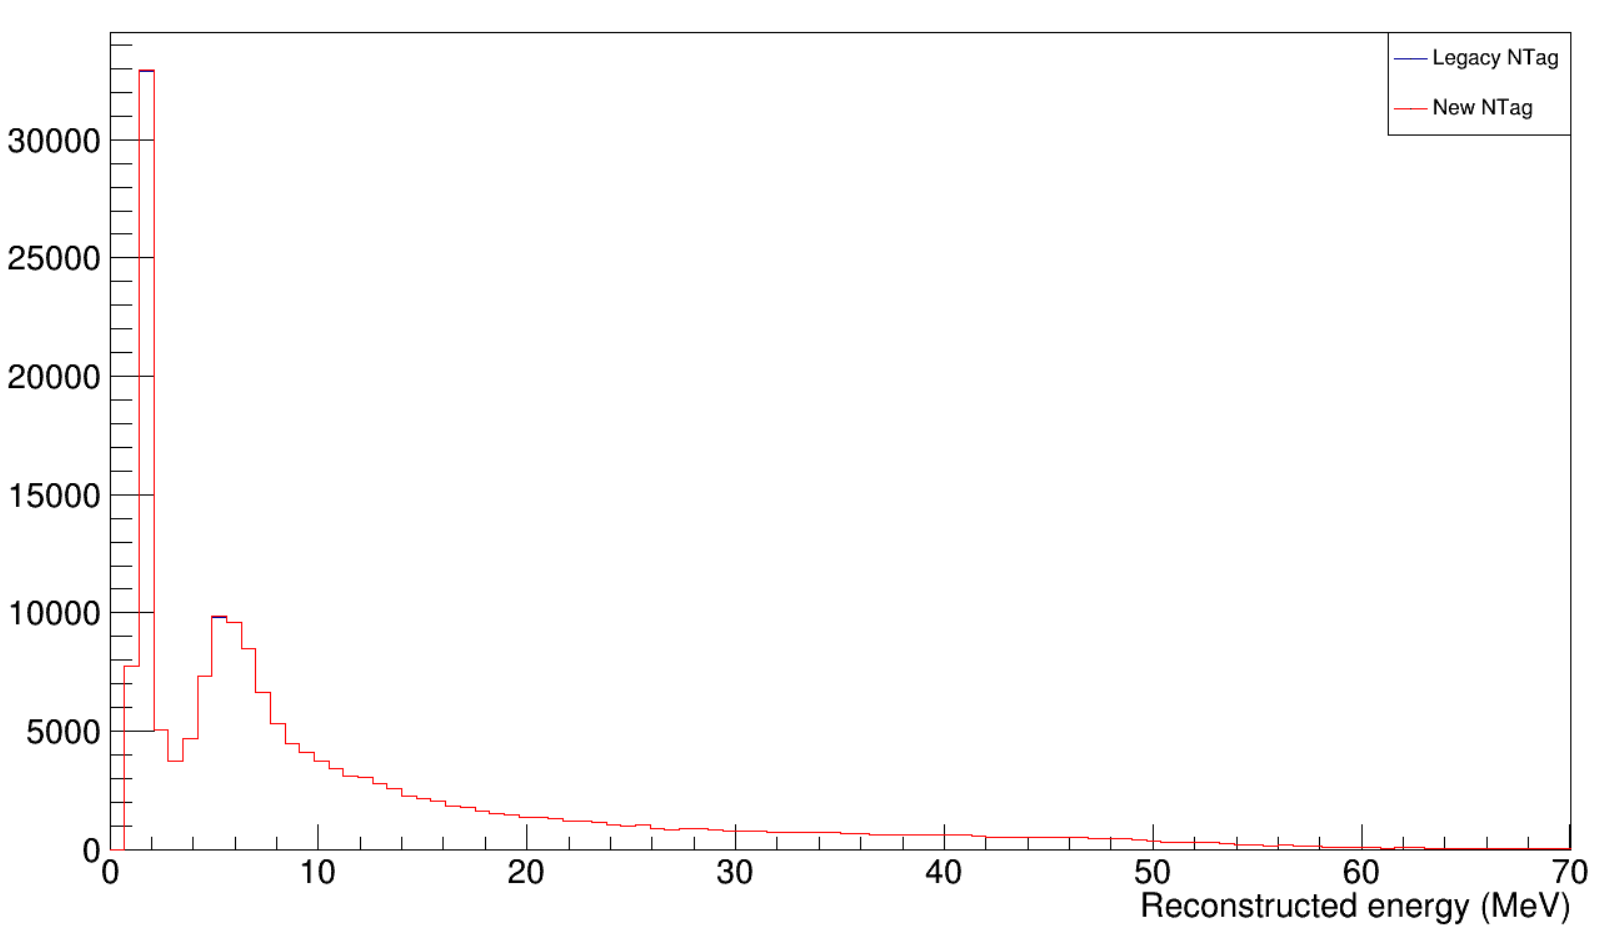
\includegraphics[width=0.9\textwidth]{Figures/energy_recon_compare.PNG}
        \caption{Reconstructed energy (MeV) comparison}
        \label{fig:energy_recon_compare}    
\end{figure}

\begin{figure}
    \centering
    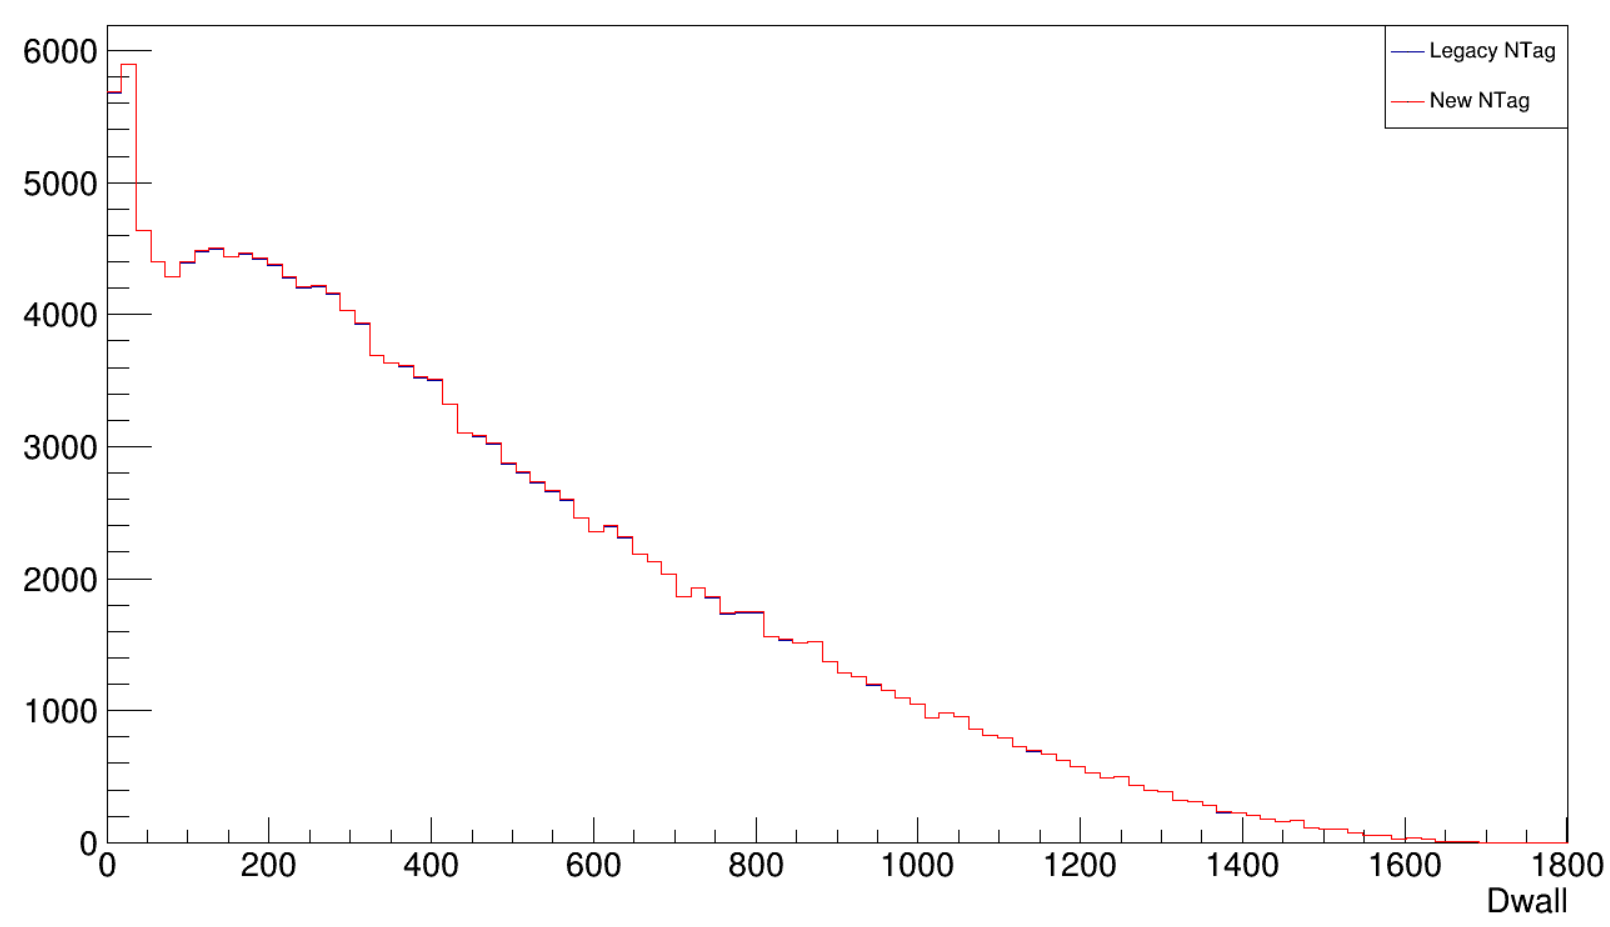
\includegraphics[width=0.9\textwidth]{Figures/dwall_recon_compare.PNG}
    \caption{DWall (cm) comparison}
    \label{fig:dwall_recon_compare}

\end{figure}

\begin{figure}
    \centering
    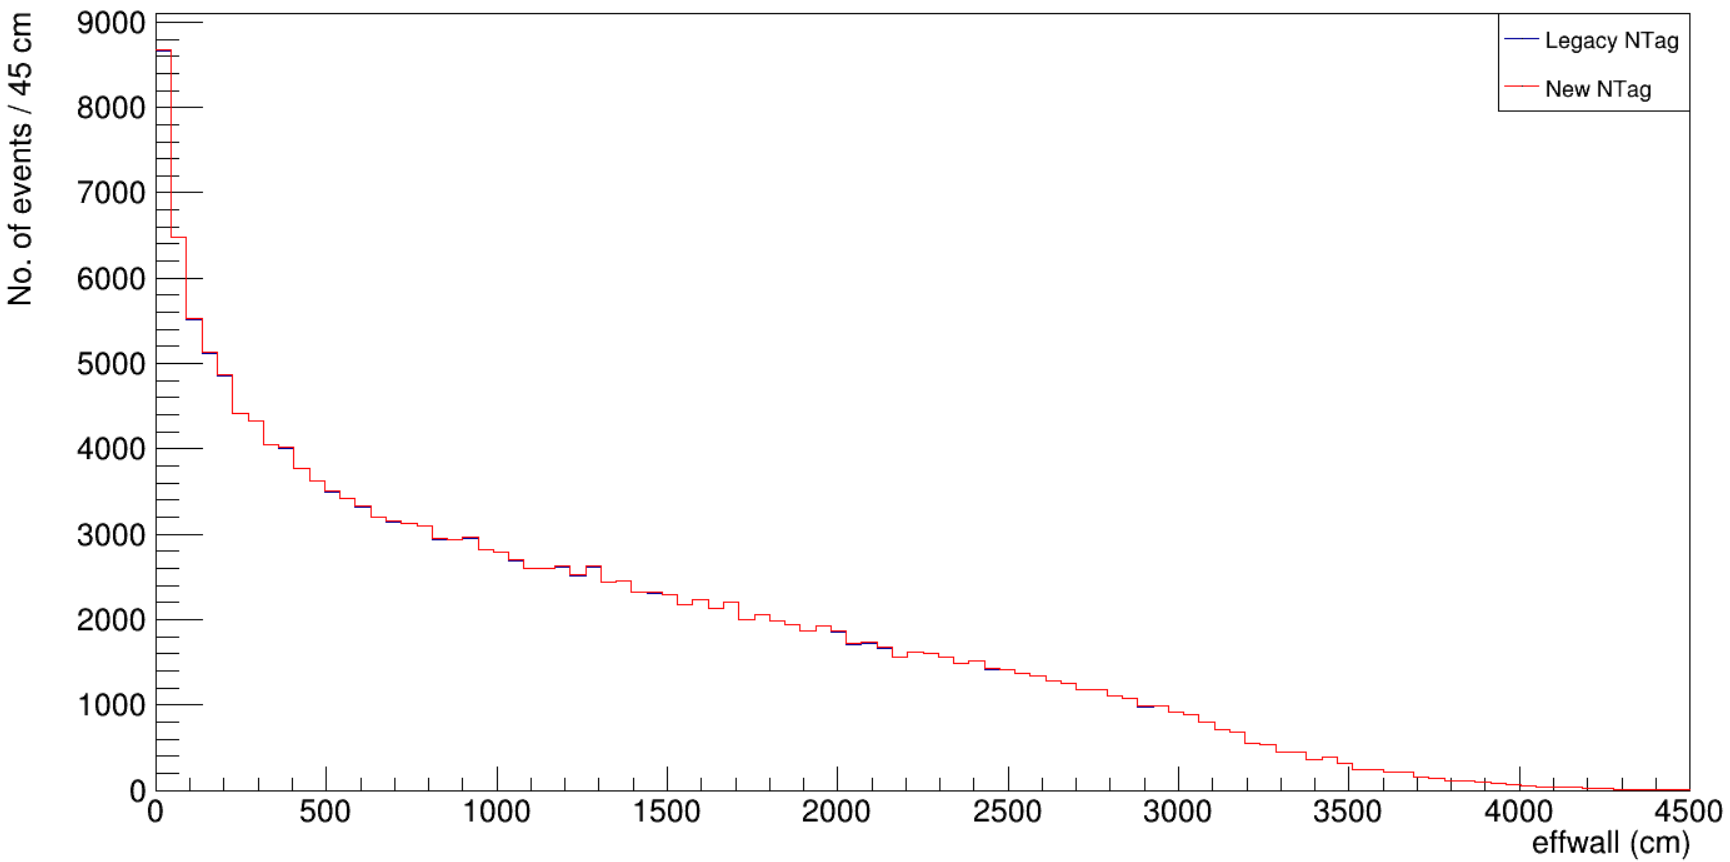
\includegraphics[width=0.9\textwidth]{Figures/effwall_recon_compare.PNG}
    \caption{Effwall (cm) comparison}
    \label{fig:effwall_recon_compare}

\end{figure}

\begin{figure}
    \centering
    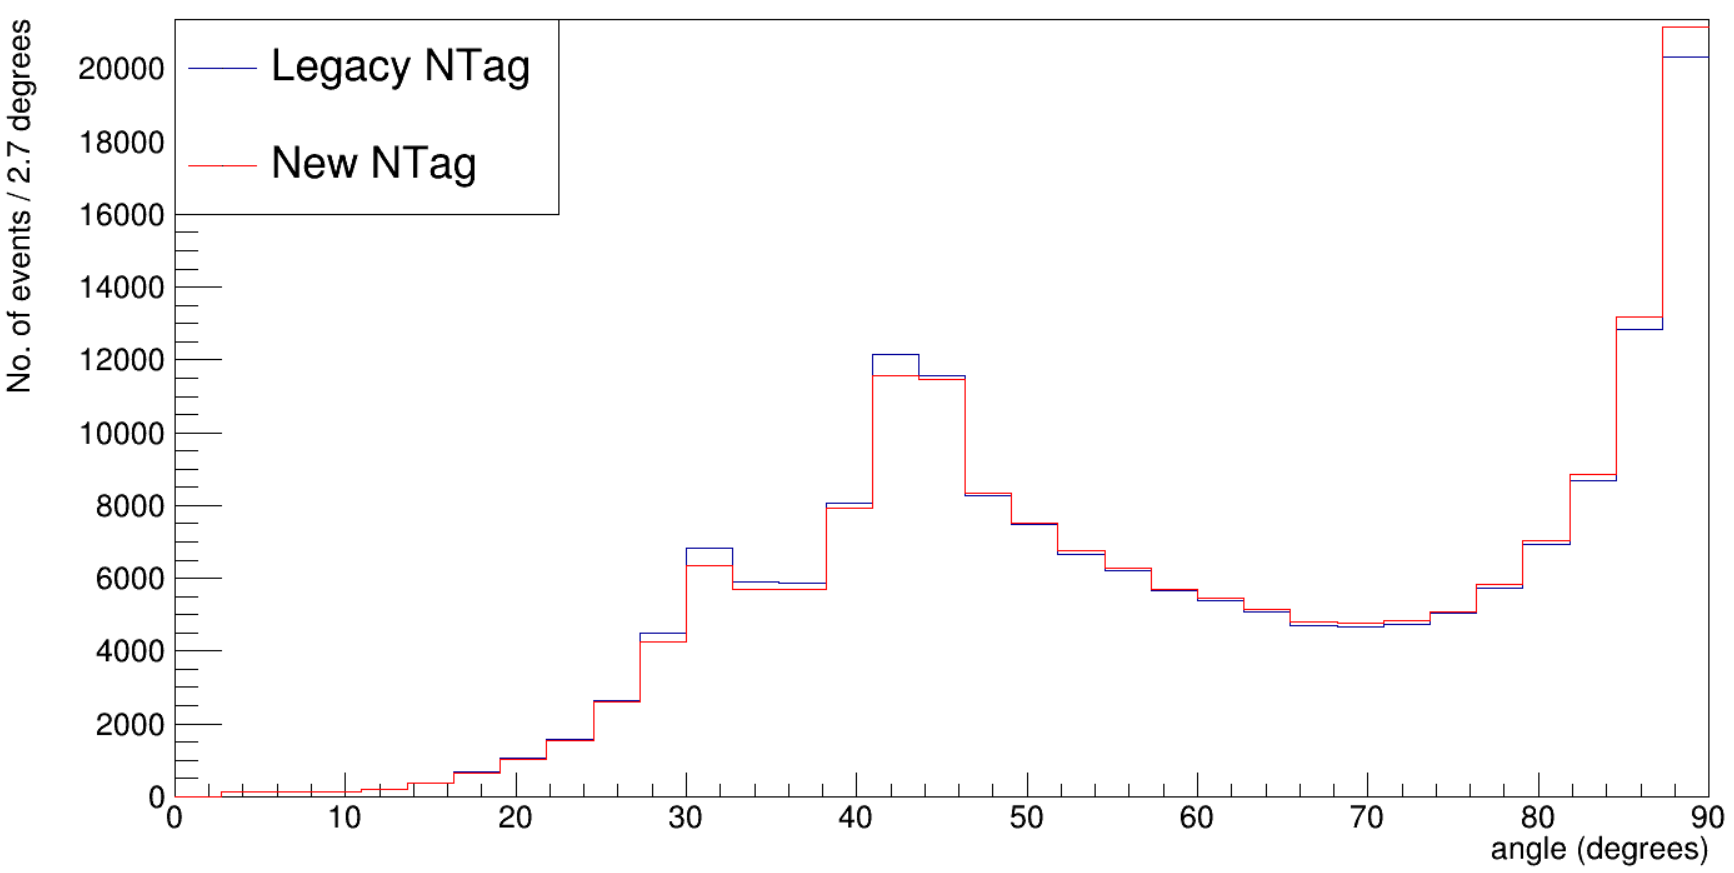
\includegraphics[width=0.9\textwidth]{Figures/angle_recon_compare.PNG}
    \caption{Reconstructed Cherenkov angle (degrees)}
    \label{fig:angle_recon_compare}

\end{figure}

\begin{figure}
    \centering
    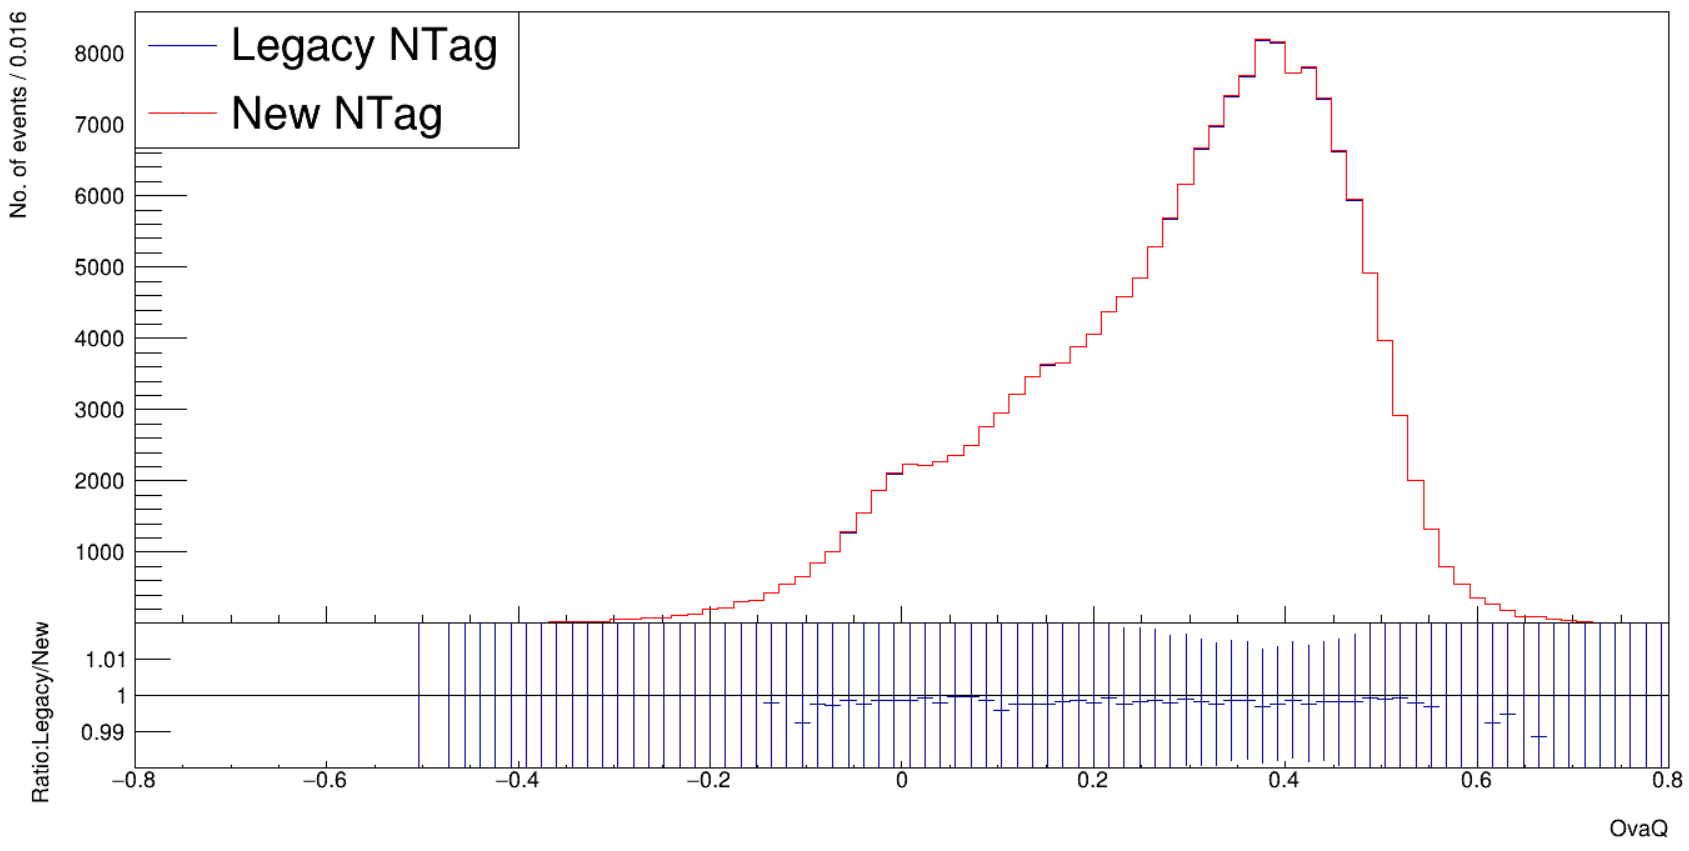
\includegraphics[width=0.9\textwidth]{Figures/ovaq_recon_compare.PNG}
    \caption{Comparisons of vertex goodness for the prompt event between versions of SKDETSIM}
    \label{fig:ovaq_recon_compare}

\end{figure}

From the comparisons of the event reconstruction variables we can conclude that there is no significant variation between the way the different gadolinium implentation models in the detector simulation doesn't affect the way the prompt event is reconstructed. This makes sense as the only difference the neutron capture model should make should relate to the secondary interactions - checking the prompt event distributions remain unchanged is a confirmation of this. Similarly, the comparisons between the two NTag versions, legacy and new show that the change in the neutron tagging algorithm didn't affect the prompt event reconstruction either. 


\subsection{NCQE event selection}

Prior to applying the neutron tagging algorithm which searches for neutron candidates, events which satisfy the neutral current quasi-elastic criteria need to be selected. This selection only involves the neutrino vertex information, no information about the neutron candidates is used in the NCQE selection process. 
\newline
The following cuts are applied to the Monte Carlo, in order to select the NCQE events. These include a visible energy cut, a fiducial volume cut, a low energy background cut, and a cut to exclude charged currrent interaction events (CCQE). 

\subsubsection{Visible energy cut}
The range for $E_{rec}$ in this variable is 3.49 MeV to 29.49 MeV - the estimated kinetic energy under the hypothesis that the event is a singular electron. The upper value for this range is chosen because the background of Michel electrons from muon neutrino and muon anti-neutrino charged current interactions increase but the NCQE signal decreases above 30 MeV. This is shown in Figure \ref{fig:michel_electron}, where the NC elastic (and therefore NCQE) signal decreases significantly above 30 MeV but the decay-e events and electron neutrino charged current events increase.

\begin{figure}
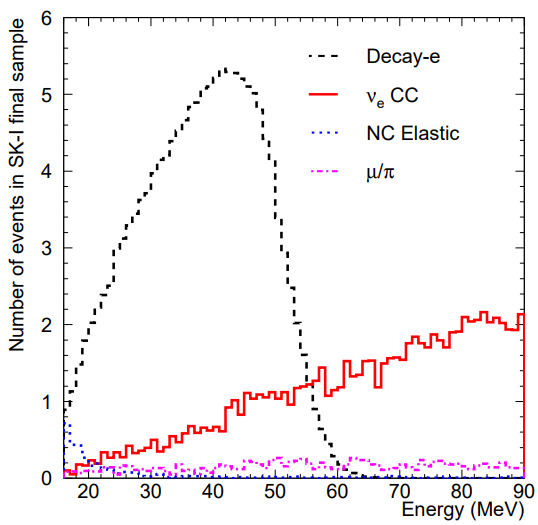
\includegraphics[width=\textwidth]{Figures/michel_electron.png}
\caption{Spectra of NCQE backgrounds where the $\nu_{\mu}$ charged current channel is from decay electron data, whereas the other three are from Monte Carlo. A clear decrease of NC elastic events are shown after 30 MeV. Taken from \cite{michel_electron}. }
\label{fig:michel_electron}
\end{figure} 

\subsubsection{Radioactivity background cut}

Due to radioactive impurities inside the detector material, specifically the wall of the inner detector, there is a cut involving the distance from the detector wall to the prompt interaction vertex - this is the fiducial volume (FV) cut. Events where the distance between the prompt interaction vertex and the detector wall is less than 200 cm are removed.

There are two more cuts used and these involve the distance to the inner detector wall. The variable dWall is defined as the distance from the reconstructed event vertex to the nearest inner detector wall inside the FV, and is set to dWall needing to be less than 200 cm.  A similar cut is also used where events where the distance between the prompt interaction vertex and the distance to the inner detector wall in the neutrino vertex vector direction (effWall) is less than 200 cm is removed. Figure \ref{fig:dwall_effwall_fv} shows an illustration of how the variables FV, dWall and effWall are defined. 

\begin{figure}
    \centering 
    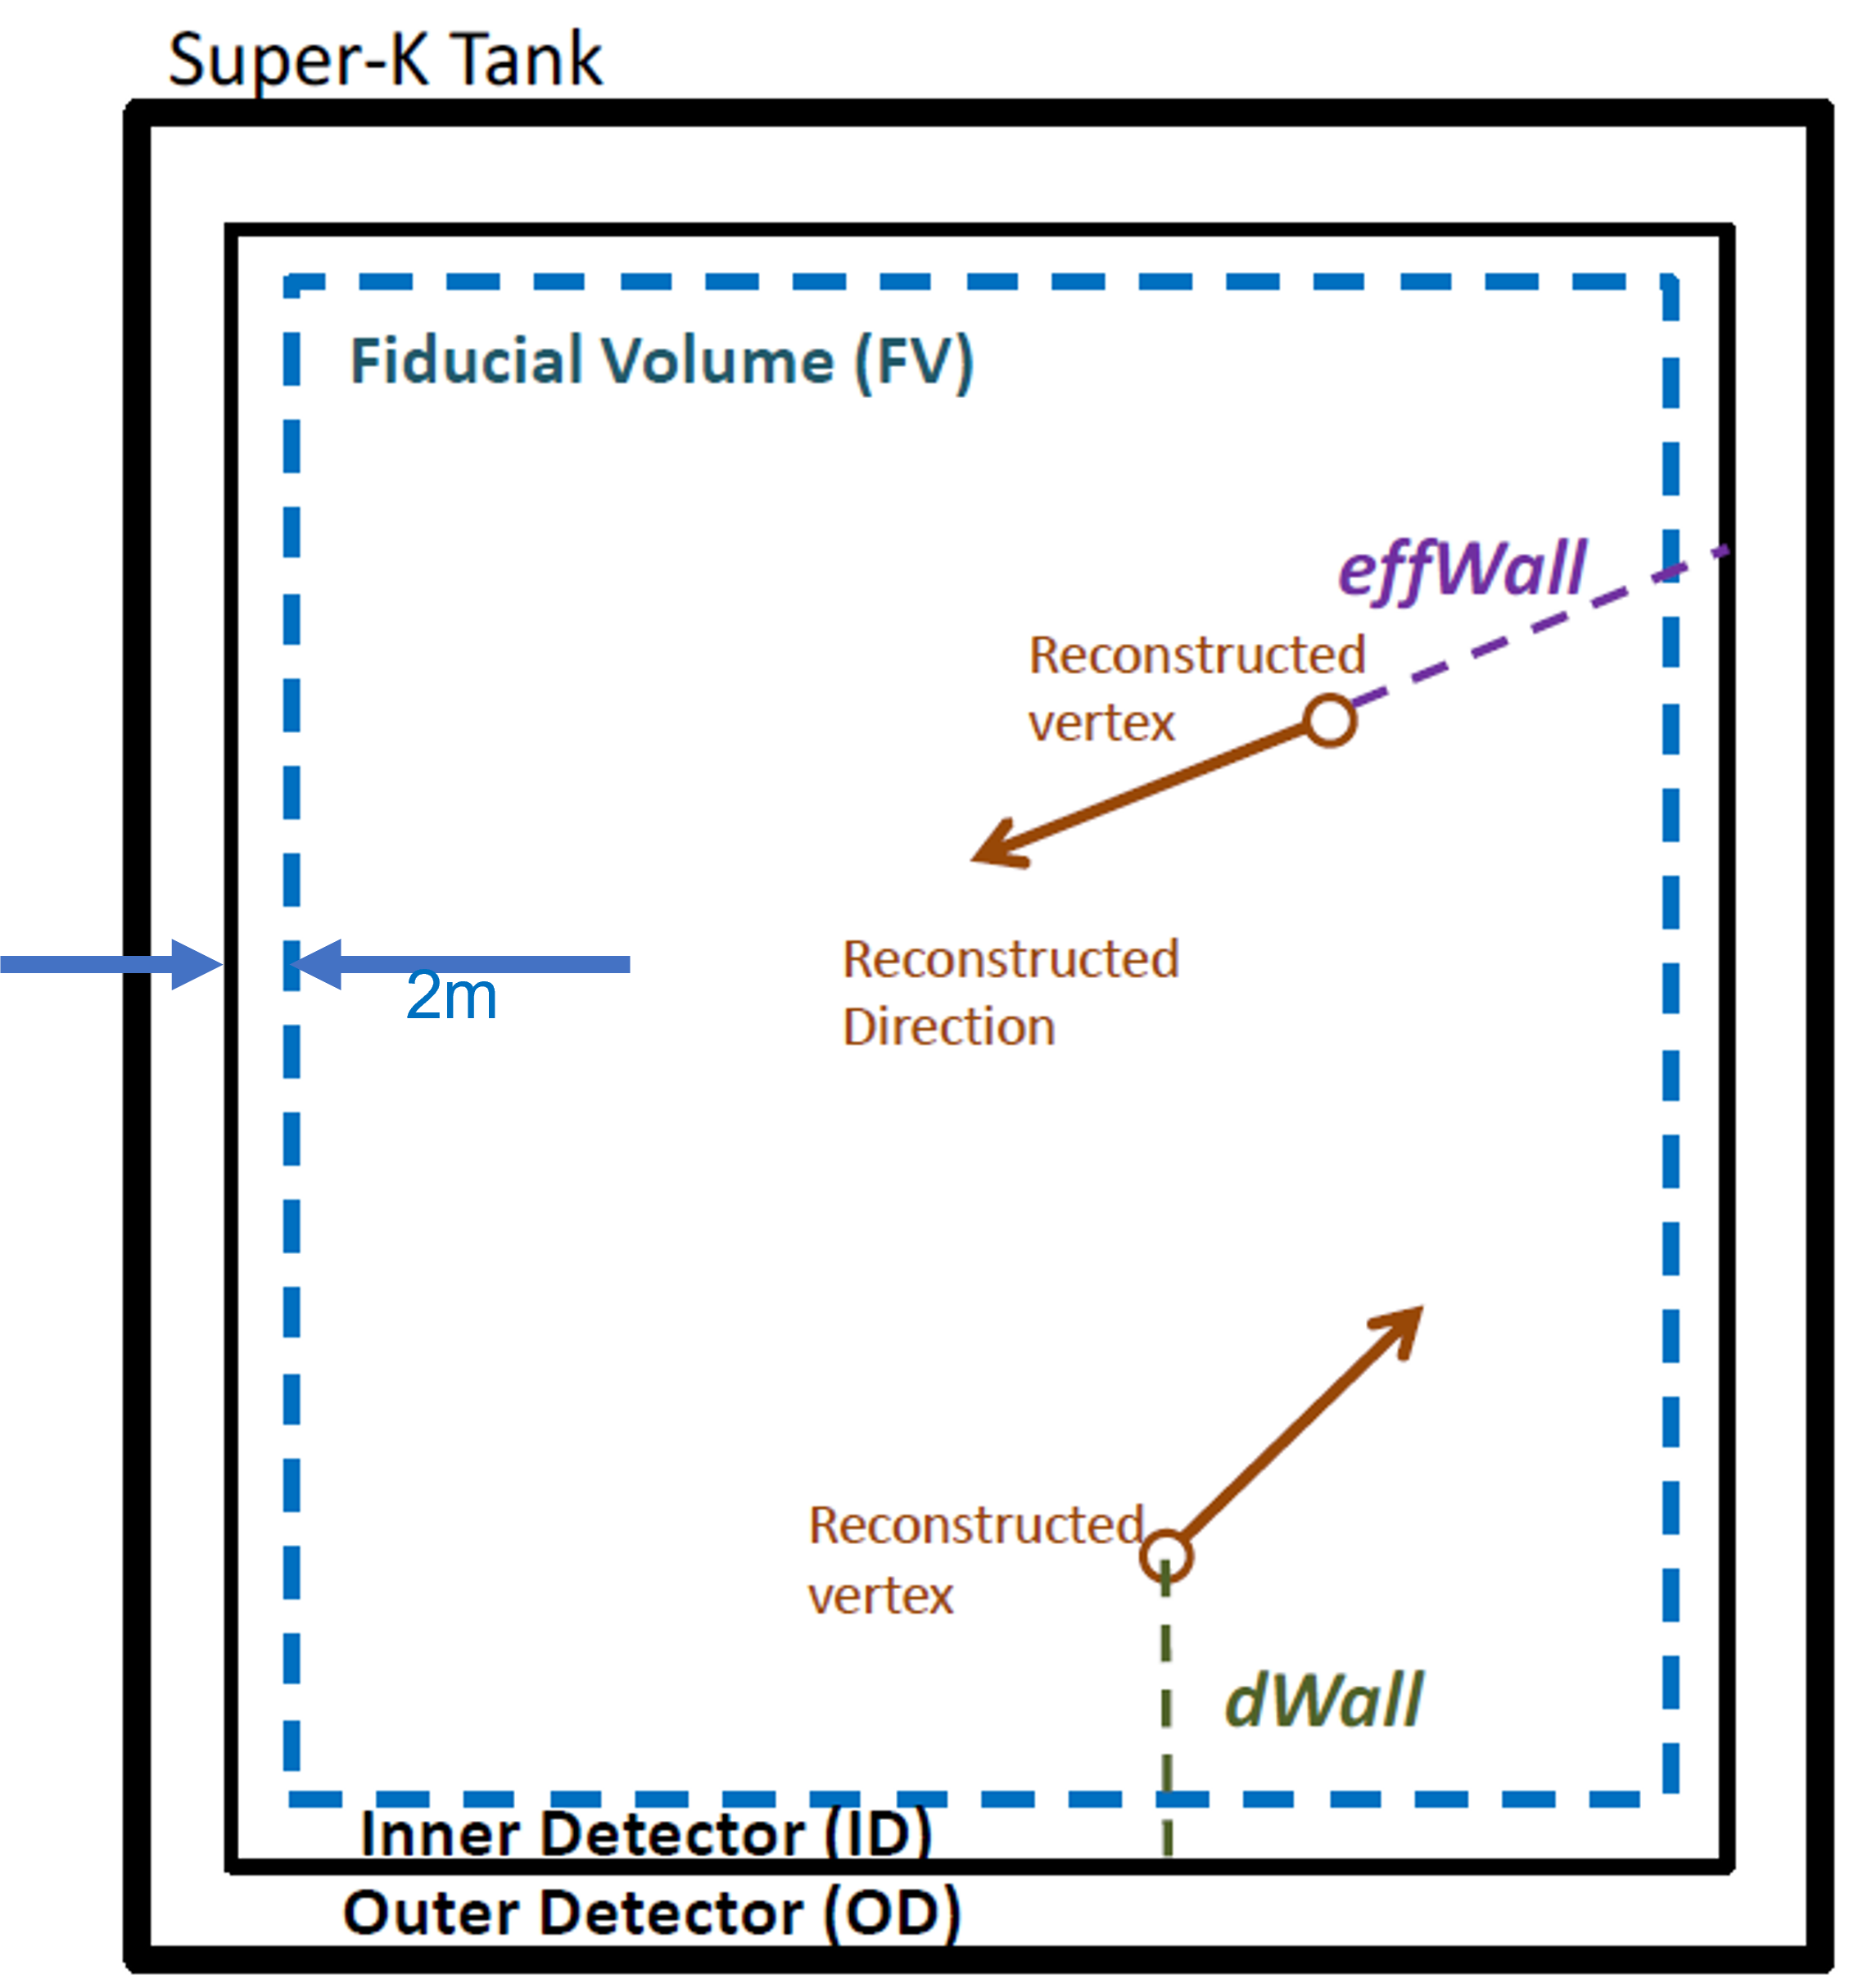
\includegraphics[width=0.6\textwidth]{Figures/fv_dwall_effwall.png}
    \caption{Schematic defining the fiducial volume (FV) and the dWall and effWall variables.}
    \label{fig:dwall_effwall_fv}
\end{figure} 
                                                                                        
These are standard cuts applied in all Super-Kamiokande analyses in order to avoid backgrounds, and when you have events where the energy region is below 6 MeV even more stringent cuts are required to further reduce background from the inner detector wall, described in the next Subsection. 

\subsubsection{Low energy background cut}

The variables dwall, effwall and ovaQ are used to tune cuts in the energy region below 6 MeV. There are five energy regions with a width of 0.5 MeV used between the lower end of the visible energy cut region (3.49 MeV) and 5.99 MeV where the cuts on the dwall, effwall and ovaQ variables are optimised. Cuts are applied on the dwall, effwall and ovaQ variables and an event is only accepted if the values of dwall, effwall and ovaQ are greater than the threshold cut values. In each 0.5 MeV energy interval, these threshold values are optimised based on the T2K run period due to the beam power and detector conditions being different from run to run, especially since the Gadolinium loading occured in the detector. Equation \ref{eq:FOM} shows how the figure-of-merit (FOM) value is to be maximised for the optimsation of each cut.

\begin{equation}
    \mathrm{FOM}=\frac{N_{\text {sig }}}{\sqrt{N_{\text {sig }}+N_{\text {bkg }}}} \quad\left(N_{\text {bkg }}=N_{\text {bkg }}^{\mathrm{MC}}+N_{\text {bkg }}^{\text {beam-unrelated }}\right)
\label{eq:FOM}
\end{equation}

Here $N_{sig}$ is the number of NCQE neutrino events in the FHC Monte Carlo sample and $N_{bkg}$ is the summation of the background events, and the FOM is calculated seperately in the five energy intervals, and the optimised cut value is taken as the one which maximises the FOM. Then the optimised cut values in each energy interval are fitted with a linear function dependent on the visible energy variables ($E_{rec}$). Equation \ref{eq:FOM_linear} gives the relation of $E_{rec}$ to the optimised cut values for dwall, effwall and ovaQ.

\begin{align}
    \text { dwall }^{\text {CUT }} =p_{0}^{\text {dwall }}+p_{1}^{\text {dwall }} \times E_{\text {rec }} \\
    \text { effwall }^{\text {CUT }}=p_{0}^{\text {effall }}+p_{1}^{\text {effwall }} \times E_{\text {rec }} \\
    \text { ova } Q^{C U T}=p_{0}^{\text {ovaQ }}+p_{1}^{\text {ovaQ }} \times E_{\text {rec }}
\label{eq:FOM_linear}
\end{align}


The scan regions and intervals for the dwall, effwall and ovaQ parameters for Equation \ref{eq:FOM_linear} are given in \cite{Abe_2019}. 

\subsection{Charged current event (CC) interaction cut}

In order to reduce the number of charged-current events which may be mistakenly included in the NCQE selection, a cut regarding the reconstructed Cherenkov angle of the prompt event  is also utilised alongside the low energy background cut, where the accepted Cherenkov angle of a prompt event ($\theta_{C}$) should be greater than the threshold cut value $\theta_{C}^{CUT}$ where the cut value is determined by the linear equation dependent on $E_{rec}$ as shown in Equation \ref{eq:thetaC_FOM}.

\begin{equation}
    \theta_{C}^{C U T}=p_{0}^{\theta_{C}}+p_{1}^{\theta_{C}} \times E_{\text {rec }}
    \label{eq:thetaC_FOM} 
\end{equation}

Just like for the low energy background cut values, the values of the optimised parameters in Equation \ref{eq:thetaC_FOM} are given in \cite{Abe_2019} and are shown in Figure \ref{fig:optimised_dwall_effwall_ovaq}.


\begin{figure}

    \begin{minipage}{.5\linewidth}
    \centering
    \subfloat[]{\label{main:a}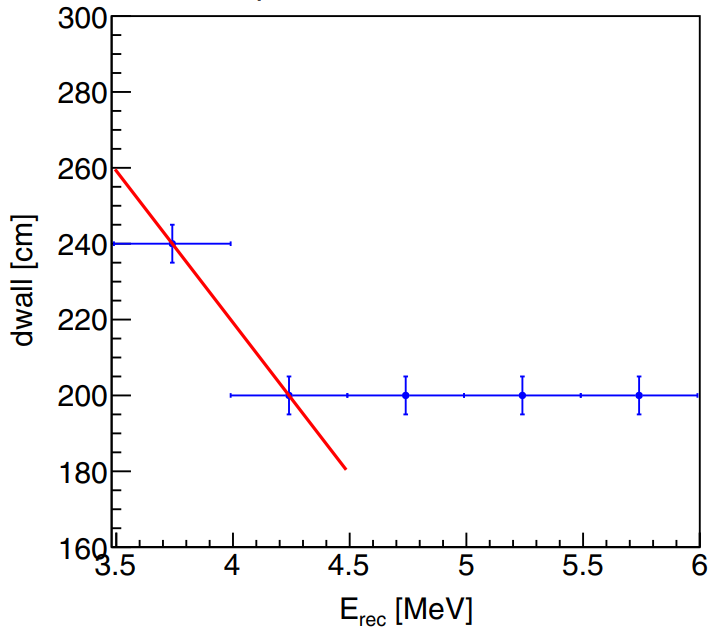
\includegraphics[scale=.5]{Figures/dwall_cut.PNG}}
    \end{minipage}%
    \begin{minipage}{.5\linewidth}
    \centering
    \subfloat[]{\label{main:b}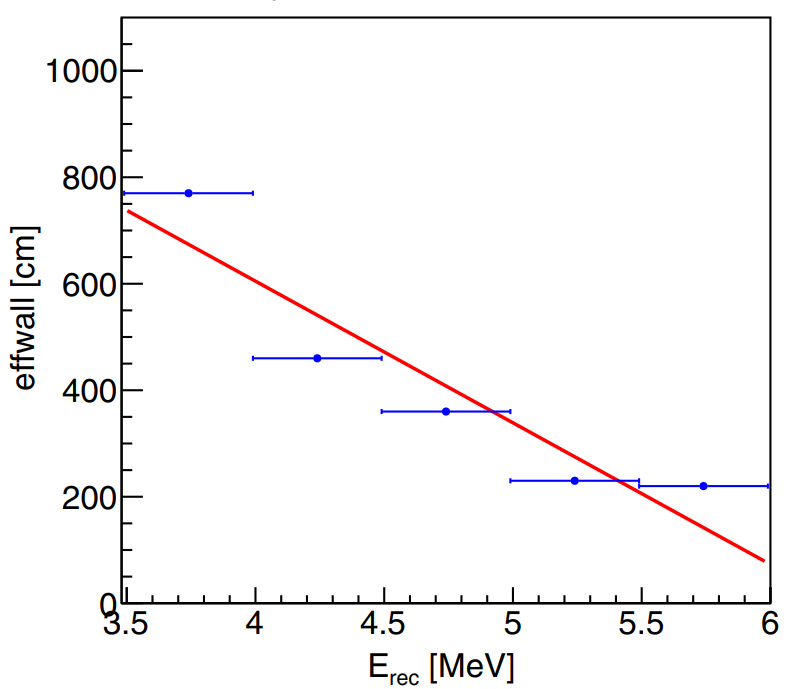
\includegraphics[scale=.5]{Figures/effwall_cut.PNG}}
    \end{minipage}\par\medskip
    \centering
    \subfloat[]{\label{main:c}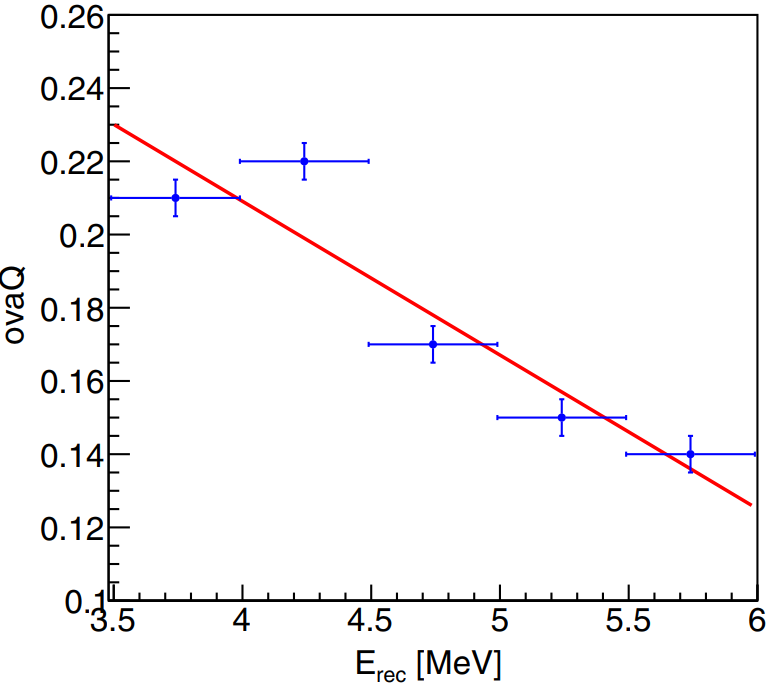
\includegraphics[scale=.5]{Figures/ovaq_cut.PNG}}
    
    \caption{Optimised cut values for dwall (top), effwall (bottom left) and ovaQ (bottom right) for Run 8 FHC mode. The red lines are linear fits to the values for these distributions, where events which have values above the lines are used in the analysis. \cite{Abe_2019}.}
    \label{fig:optimised_dwall_effwall_ovaq}
\end{figure}
    


\subsection{Prompt event NCQE reduction cut plots}

Before applying the NTag algorithm, either legacy or new, plots were produced of the number of neutrino events and their dependence the reduction cut variables mentioned previously. These are shown in Figures \ref{fig:erec_reduction} to \ref{fig:angle_reduction}. Each figure shows the corresponding plot for the previous NCQE analysis carried out with neutron tagging on Hydrogen on the left, with the plot from this analysis on the right. Due to the FHC sample not purely consisting of neutrino and antineutrino NCQE interactions, Table \ref{table:nu_FHC_mc} gives the expected number of neutrino events for each type of interaction including neutral current and charged current interactions.

\begin{table}
    $$
    \begin{array}{ccc}
    \hline \text { FHC sample } & \text { MC } \# \boldsymbol{\nu}_{\text {det }} & \text { MC } \# \nu_{\text {det }} \text { fraction (\%) } \\
    \hline \nu-N C Q E & 204.1 & 76.6 \\
    \bar{\nu}-\text { NCQE } & 5.6 & 2.1 \\
    N C-\text { other } & 47.8 & 17.9 \\
    C C & 8.8 & 3.3 \\
    \hline \text { Total } & 266.3 & 100 \\
    \hline
    \end{array}
    $$
    \caption{FHC MC expectation values for each interaction type}
    \label{table:nu_FHC_mc}
\end{table}


\begin{figure}[!htbp]
    \centering
    
    \caption{Comparisons of stacked histrograms for the $E_{rec}$ variable between NCQE neutron tag on H analysis (left) and this analysis (right)} \label{fig:erec_reduction} 
    
    \subfloat[]{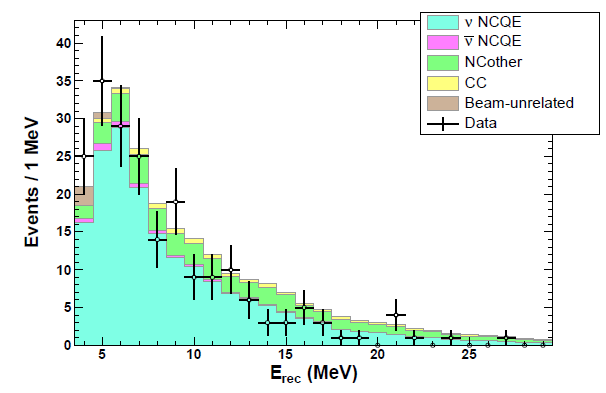
\includegraphics[width=0.49\textwidth]{Figures/fabio_erec.PNG}}  \hfill 
    \subfloat[]{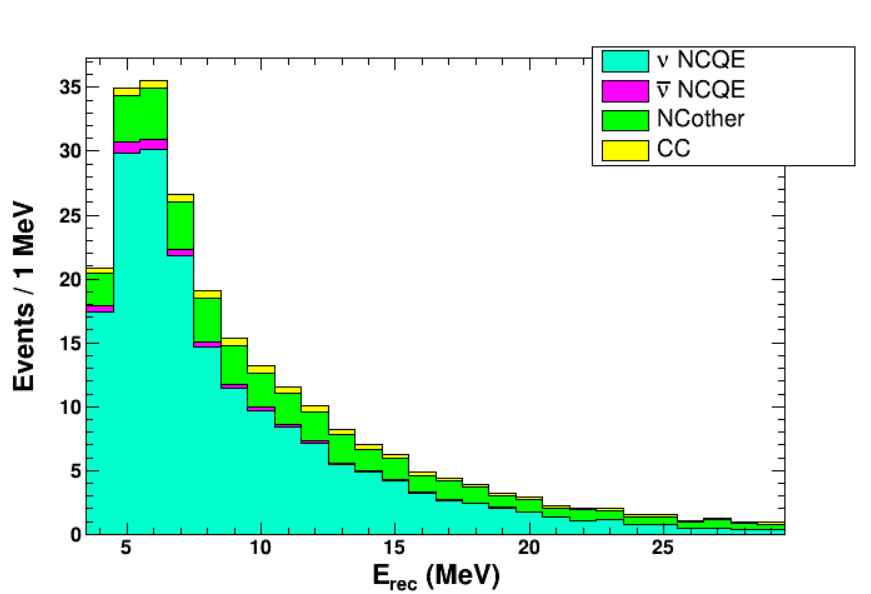
\includegraphics[width=0.49\textwidth]{Figures/erec_reduction.PNG}} \par
    
        
\end{figure}

\begin{figure}[!htbp]
    \centering
    
    \caption{Comparisons of stacked histrograms for the Dwall variable between NCQE neutron tag on H analysis (left) and this analysis (right)} \label{fig:dwall_reduction} 
    
    \subfloat[]{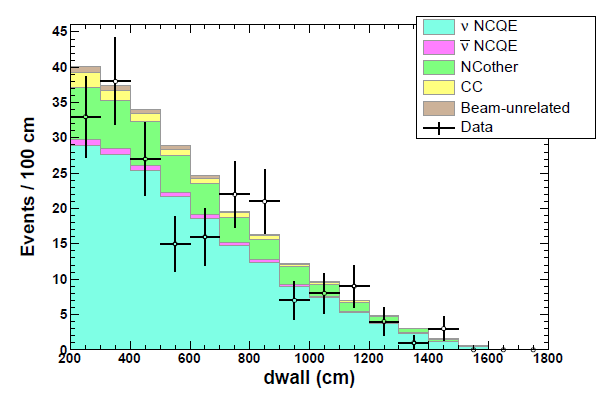
\includegraphics[width=0.49\textwidth]{Figures/fabio_dwall.PNG}}  \hfill 
    \subfloat[]{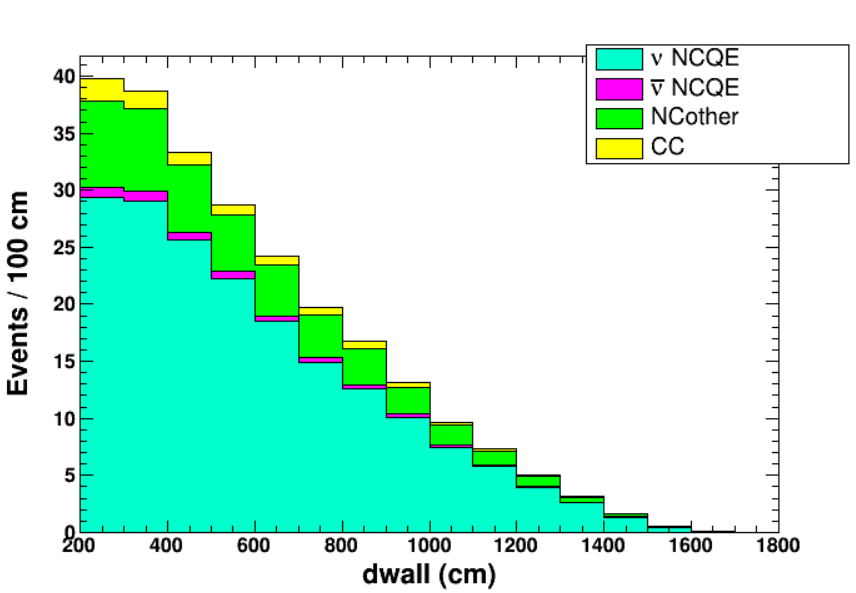
\includegraphics[width=0.49\textwidth]{Figures/dwall_reduction.PNG}}  \par
    
        
\end{figure}

\begin{figure}[!htbp]
    \centering
    
    \caption{Comparisons of stacked histograms for the Effwall variable between NCQE neutron tag on H analysis (left) and this analysis (right)} \label{fig:effwall_reduction} 
    
    \subfloat[]{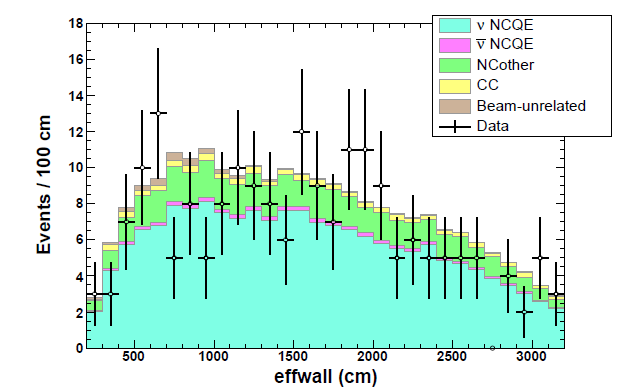
\includegraphics[width=0.49\textwidth]{Figures/fabio_effwall.PNG}}  \hfill 
    \subfloat[]{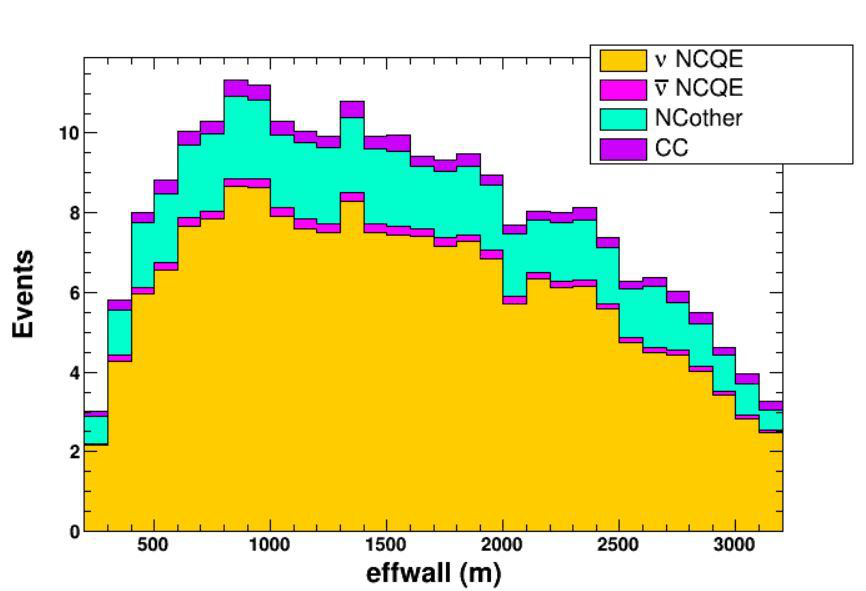
\includegraphics[width=0.49\textwidth]{Figures/effwall_reduction.PNG}} \par
    
        
\end{figure}

\begin{figure}[!htbp]
    \centering
    
    \caption{Comparisons of stacked histrograms for the ovaQ variable between NCQE neutron tag on H analysis (left) and this analysis (right)} \label{fig:ovaq_reduction} 
    
    \subfloat[]{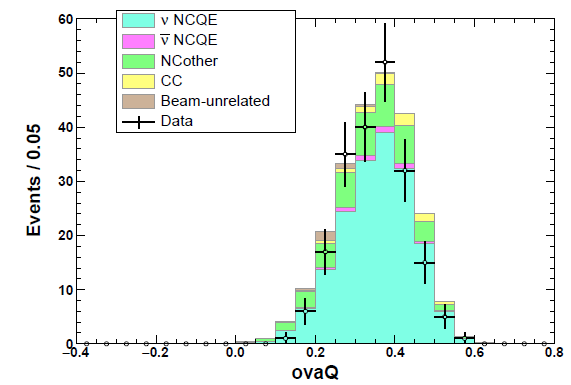
\includegraphics[width=0.49\textwidth]{Figures/fabio_ovaq.PNG}} \hfill 
    \subfloat[]{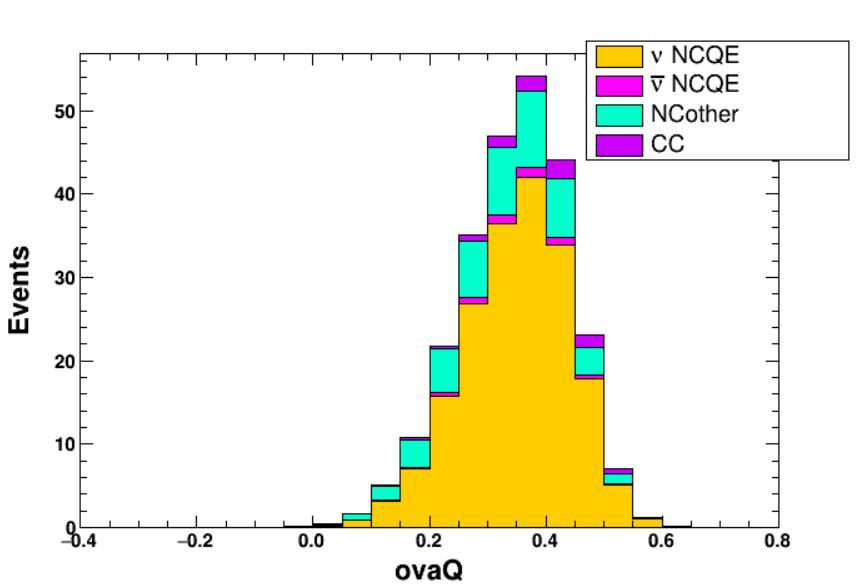
\includegraphics[width=0.49\textwidth]{Figures/ovaq_reduction.PNG}} \par
    
        
\end{figure}

\begin{figure}[!htbp]
    \centering
    
    \caption{Comparisons of stacked histograms for the $\theta_C$ variable between NCQE neutron tag on H analysis (left) and this analysis (right)} \label{fig:angle_reduction} 
    
    \subfloat[]{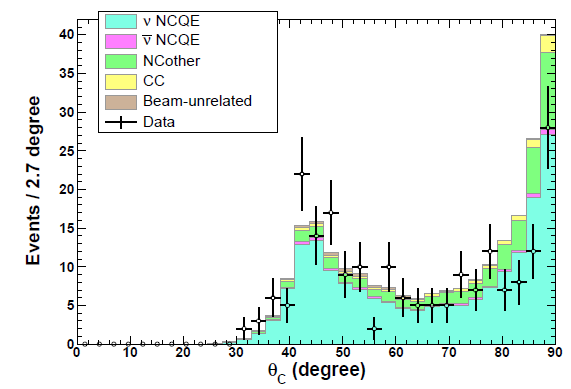
\includegraphics[width=0.49\textwidth]{Figures/fabio_angle.PNG}} \hfill 
    \subfloat[]{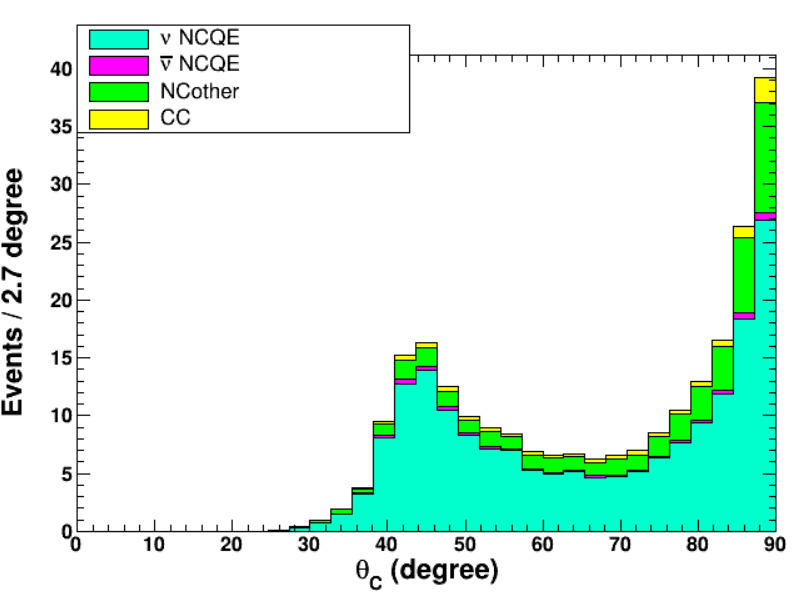
\includegraphics[width=0.49\textwidth]{Figures/angle_reduction.PNG}} \par
    
        
\end{figure}



\section{Secondary selection}

As mentioned previously, two neutron tagging algorithms were used in this analysis, the legacy NTag code, used in previous NCQE analyses and modified to work with a version of SKDETSIM which has Gadolinium included and new NTag code which uses a slightly different neutron tagging algorithm specifically with regards to the primary and secondary selection criteria which will be discussed in later subsections.



\subsection{True neutron tagging information}

Prior to defining the primary and secondary selection criteria for each neutron tagging algorithm, it is important to produce some distributions of basic variables regarding the neutron capture that occur in the simulation, such as neutron capture time, position and number. Figure \ref{fig:NCapTime} shows the distribution for the number of neutron captures and the true capture time of the neutrons for both the legacy (green) and new (red) NTag code.  

\begin{figure}
    \centering
     \begin{subfigure}[b]{0.49\linewidth}
      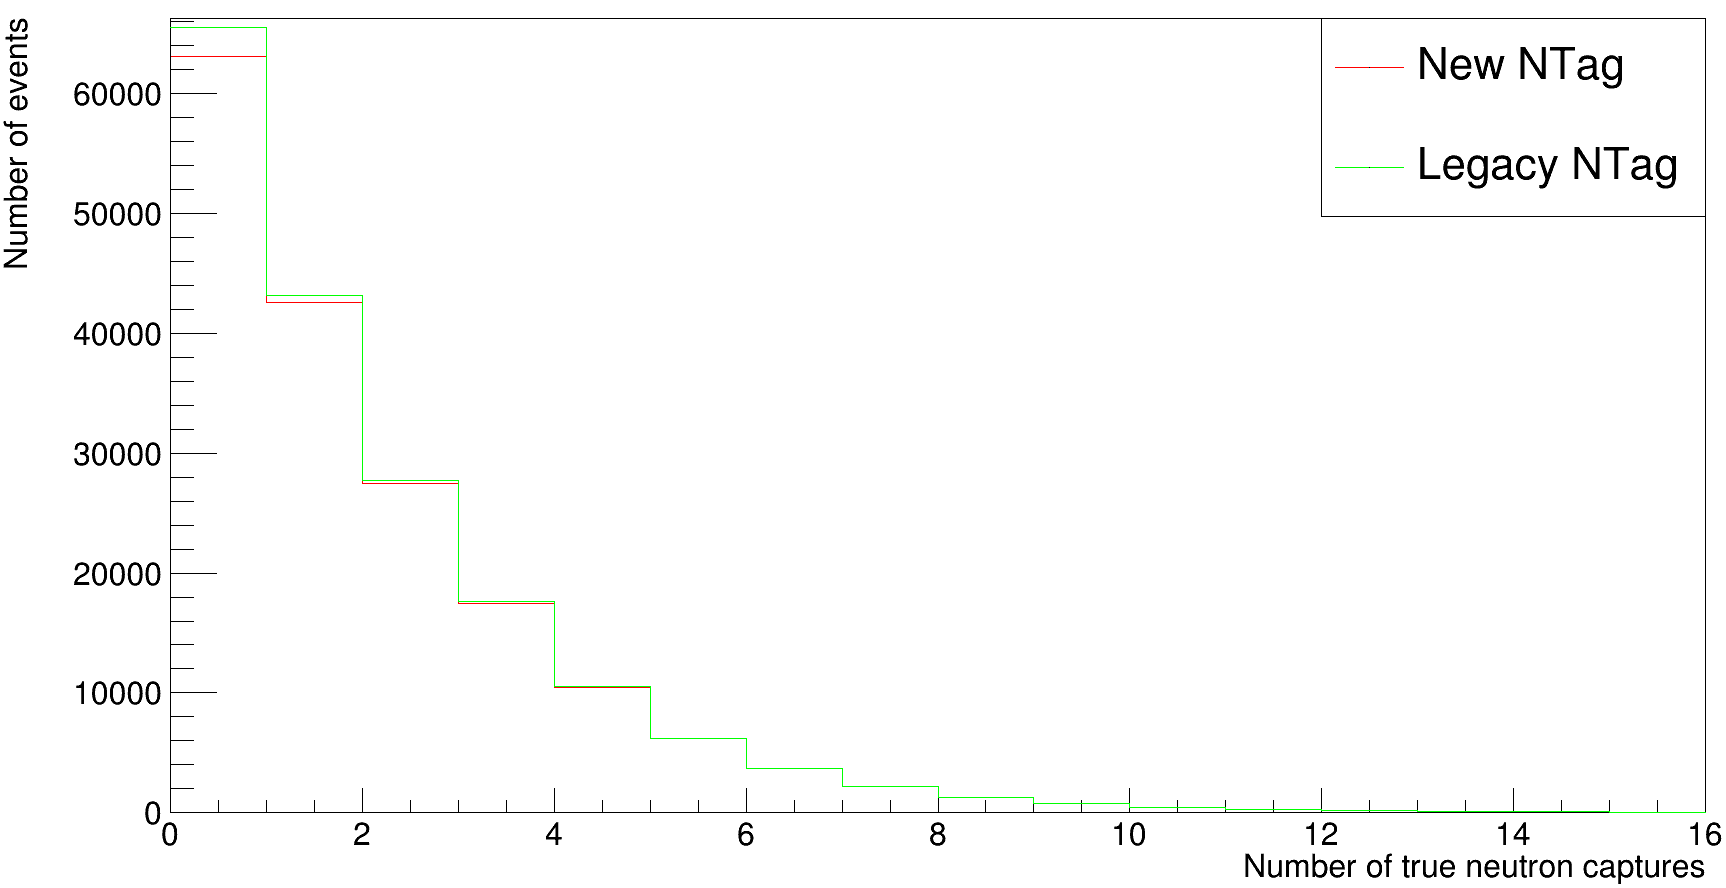
\includegraphics[width=\linewidth]{Figures/NTrueCaptures.PNG}
     \end{subfigure}
     \begin{subfigure}[b]{0.49\linewidth}
       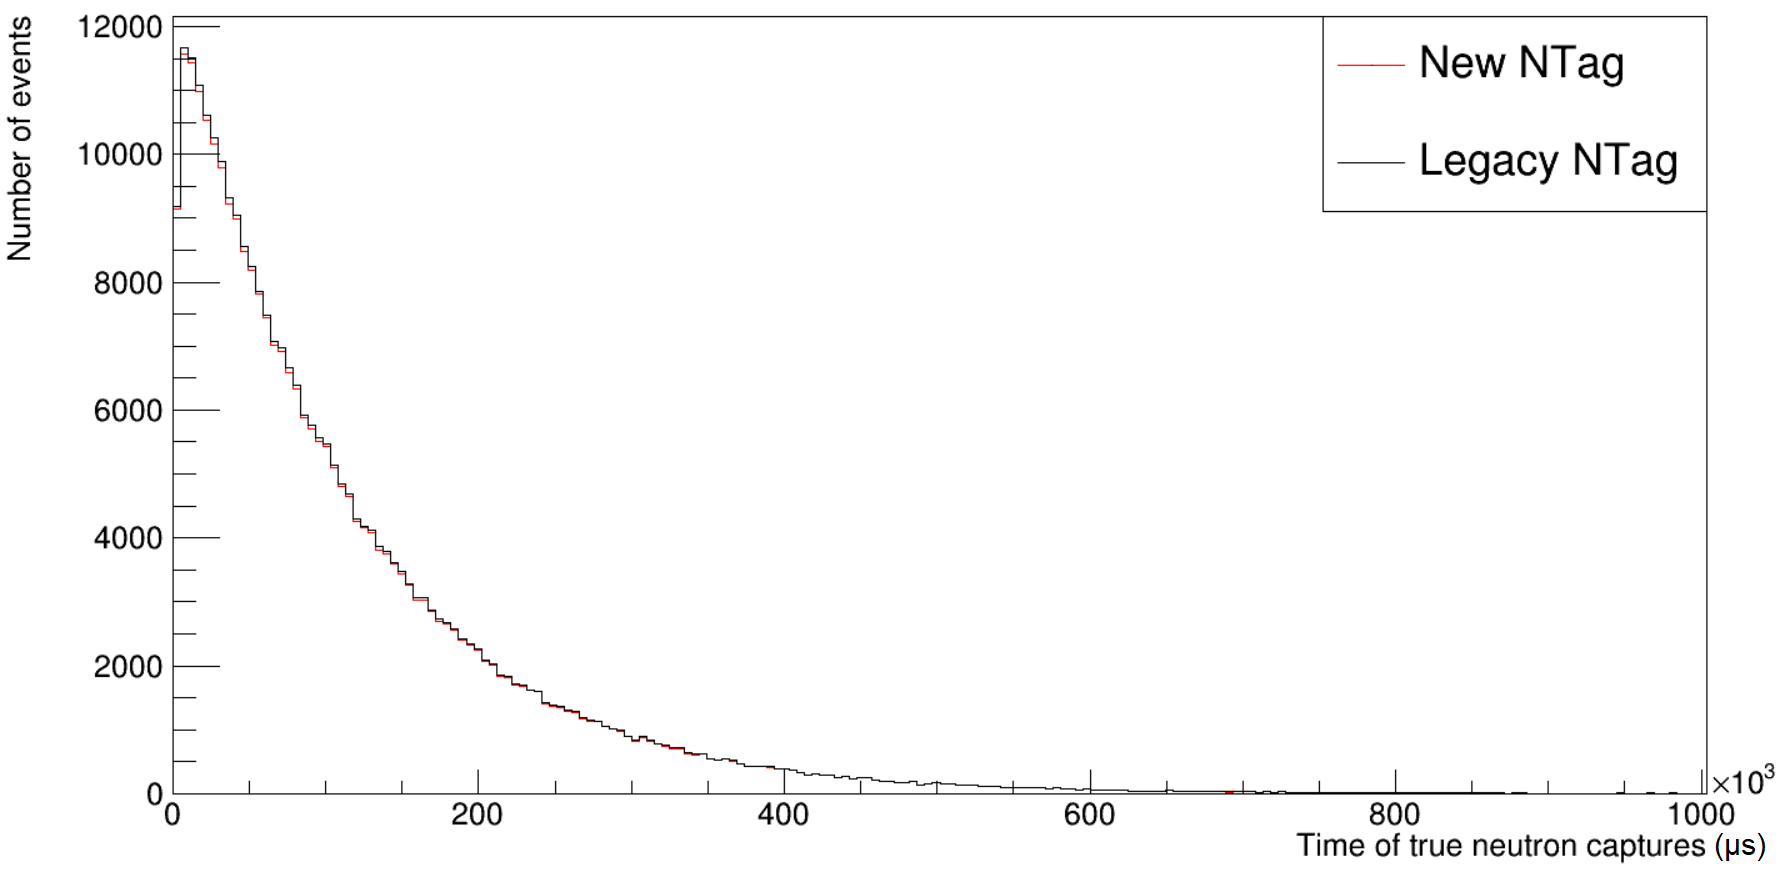
\includegraphics[width=\linewidth]{Figures/TrueCaptureTime.PNG}
      \end{subfigure} 
      \caption{Number of events plotted against number of true neutron captures (left) and number of events plotted against the time of all neutron captures ($\mu$s) (right). }
      \label{fig:NCapTime}
\end{figure}

In order to classify the neutron captures on hydrogen and gadolinium seperately, the energy of the gammas produced from the neutron capture were used, along with the number of gammas produced from the neutron capture. If the energy of the gamma produced is 2.22 MeV and only one gamma ray was produced from the neutron capture, the neutron capture was classified as a capture on a proton. If there are multiple gamma rays produced and if the energy of the gamma cascade is 8.5 MeV in total it is classified as a neutron capture on ${ }^{155} \mathrm{Gd}$ and if the energy of the gamma cascade is 7.9 MeV, it is classified as a neutron capture on ${ }^{157} \mathrm{Gd}$. Distributions of the number of gammas produced from neutron capture in the simulation, and also the energy of these gammas were plotted, shown for both the legacy (green) and new (red) NTag code, shown in Figure \ref{fig:GammaPlots}. 

\begin{figure}
    \centering
     \begin{subfigure}[b]{0.49\linewidth}
      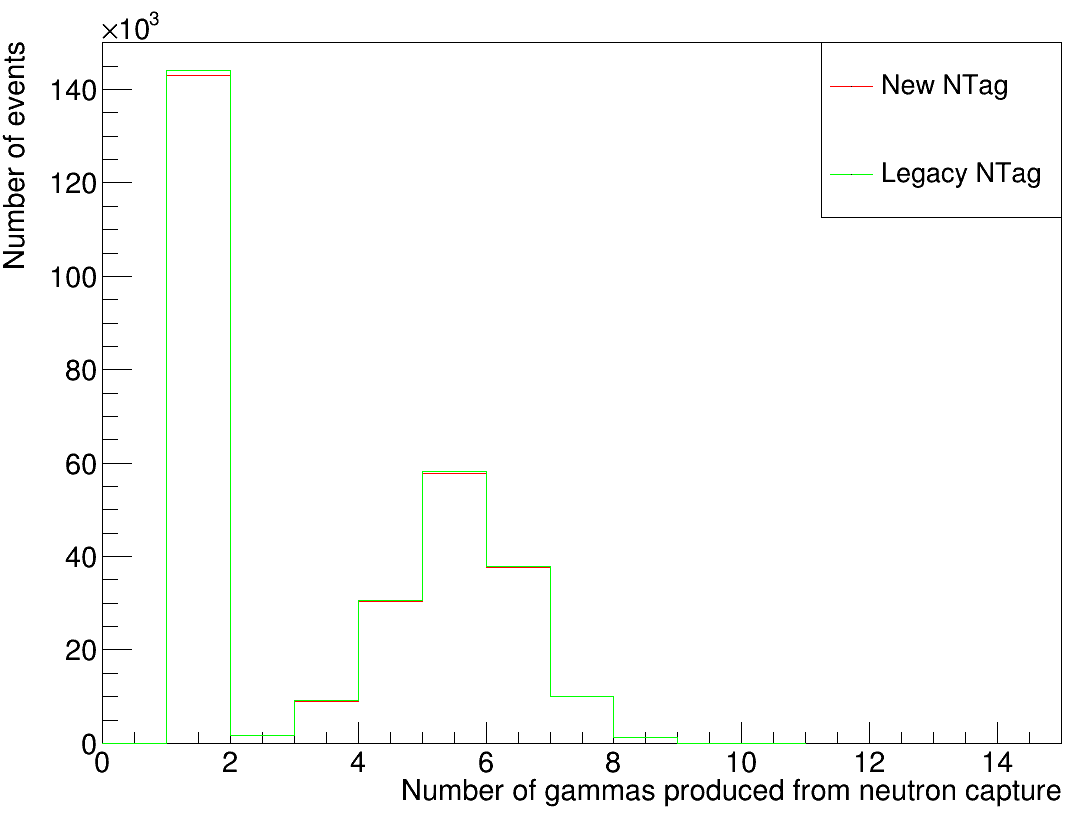
\includegraphics[width=\linewidth]{Figures/NGamma.PNG}
     \end{subfigure}
     \begin{subfigure}[b]{0.49\linewidth}
       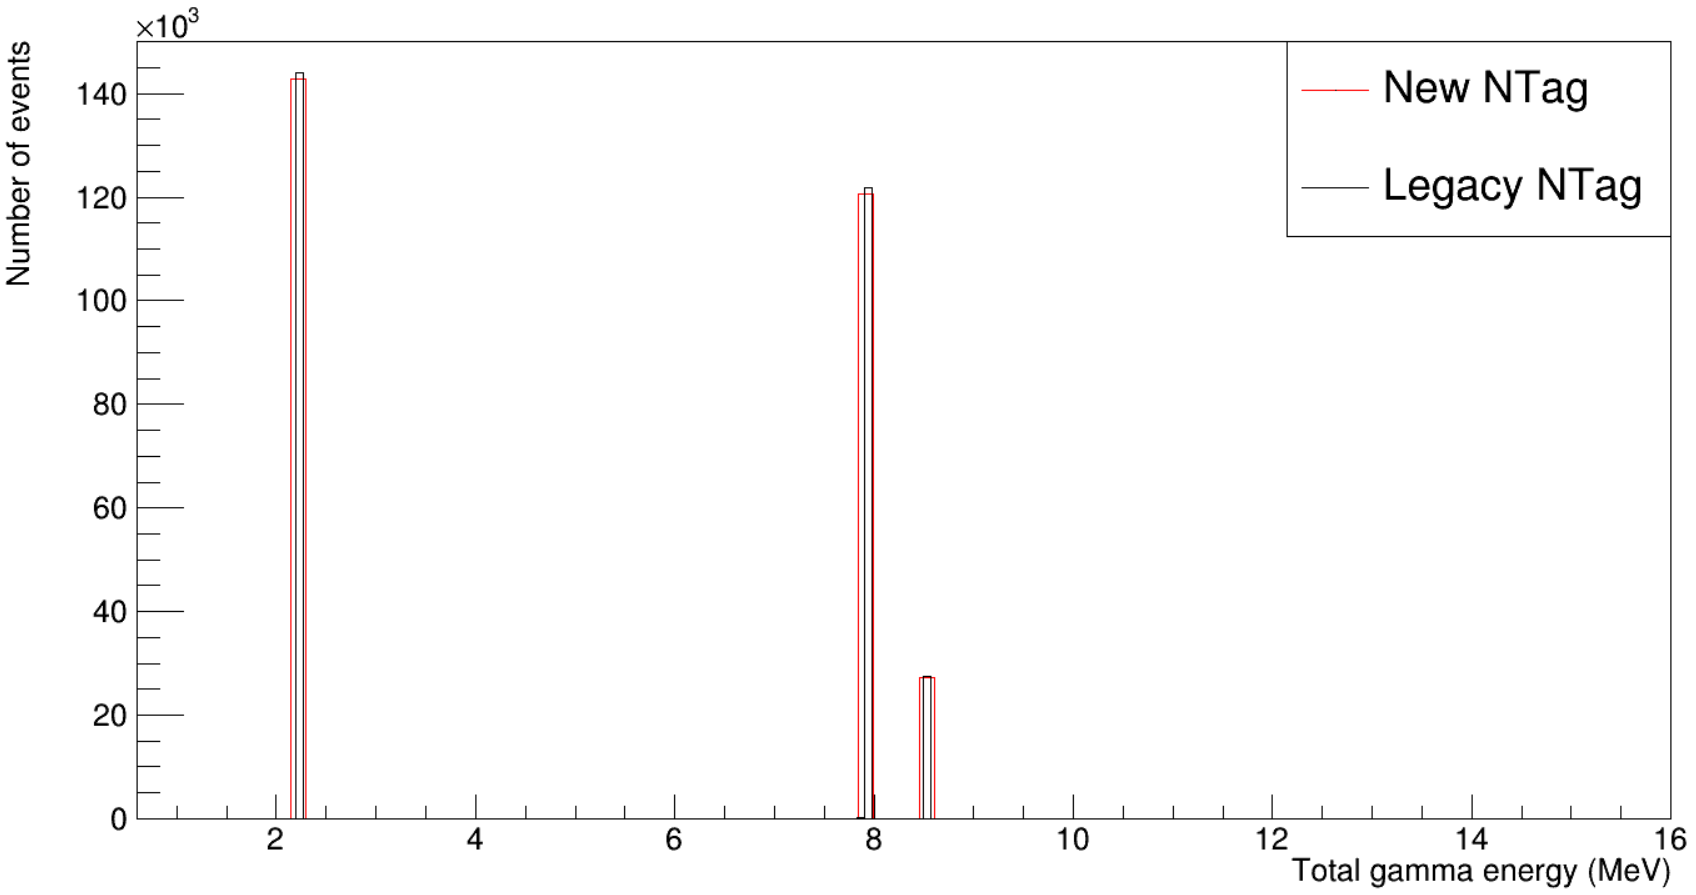
\includegraphics[width=\linewidth]{Figures/TotGammaE.PNG}
      \end{subfigure} 
      \caption{Number of gamma rays produced by neutron capture (left) and total energy of gamma rays produced by neutron capture (right) in the Monte Carlo}
      \label{fig:GammaPlots}
\end{figure}

Figure \ref{fig:GammaPlots} shows that both NTag algorithms have the same number of gammas produced by neutron capture on hydrogen (shown by the peak at 2.22 MeV), and the same number of gammas for the gamma cascade produced by neutron capture on the ${ }^{155} \mathrm{Gd}$ and 
${ }^{157} \mathrm{Gd}$ isotopes of Gadolinium, where the modal number of gammas in the cascade for both NTag code is five. In addition to checking the number and energy of the gammas, and the number and time of true neutron captures, the neutron capture positions for the x,y and z directions were also plotted as shown in \ref{fig:TrueNCapPos}.

\begin{figure}
\centering
    \begin{minipage}{0.5\linewidth}
    \subfloat[]{\label{main:a}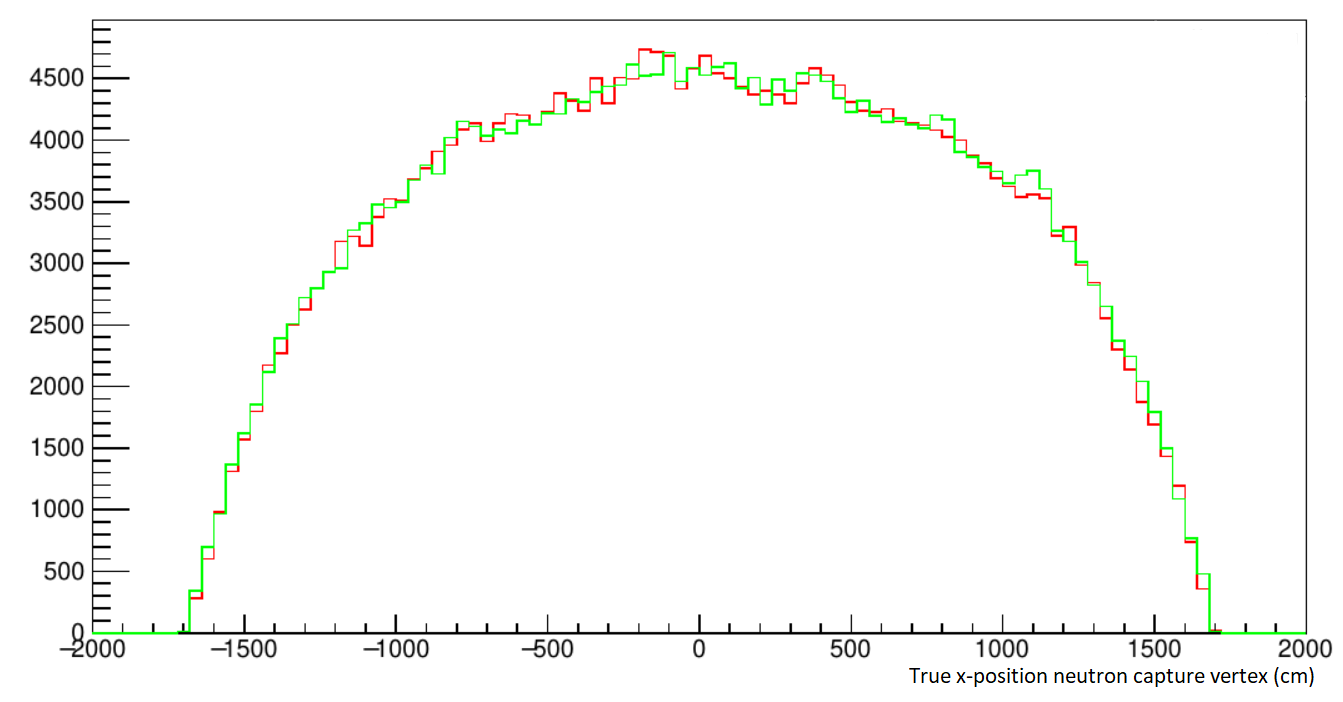
\includegraphics[scale=0.3]{Figures/xTrueCapturePos.png}}
    \end{minipage}%
    \begin{minipage}{0.5\linewidth}
    \centering
    \subfloat[]{\label{main:b}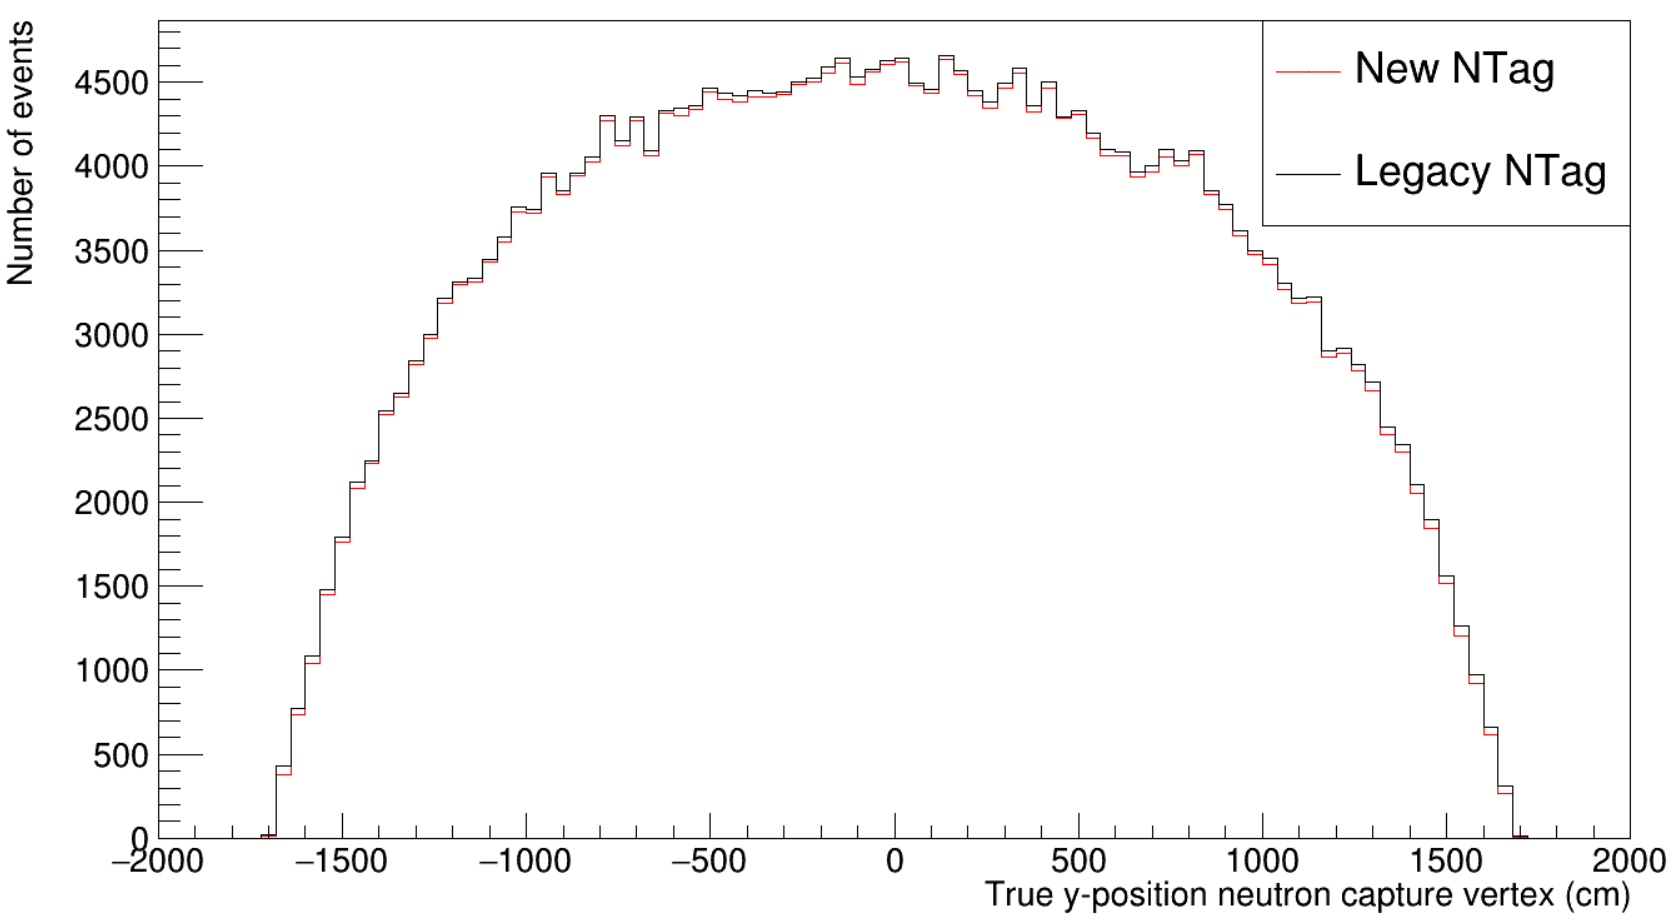
\includegraphics[scale=0.3]{Figures/yTrueCapturePos.png}}
    \end{minipage}\par\medskip
    \centering
    \subfloat[]{\label{main:c}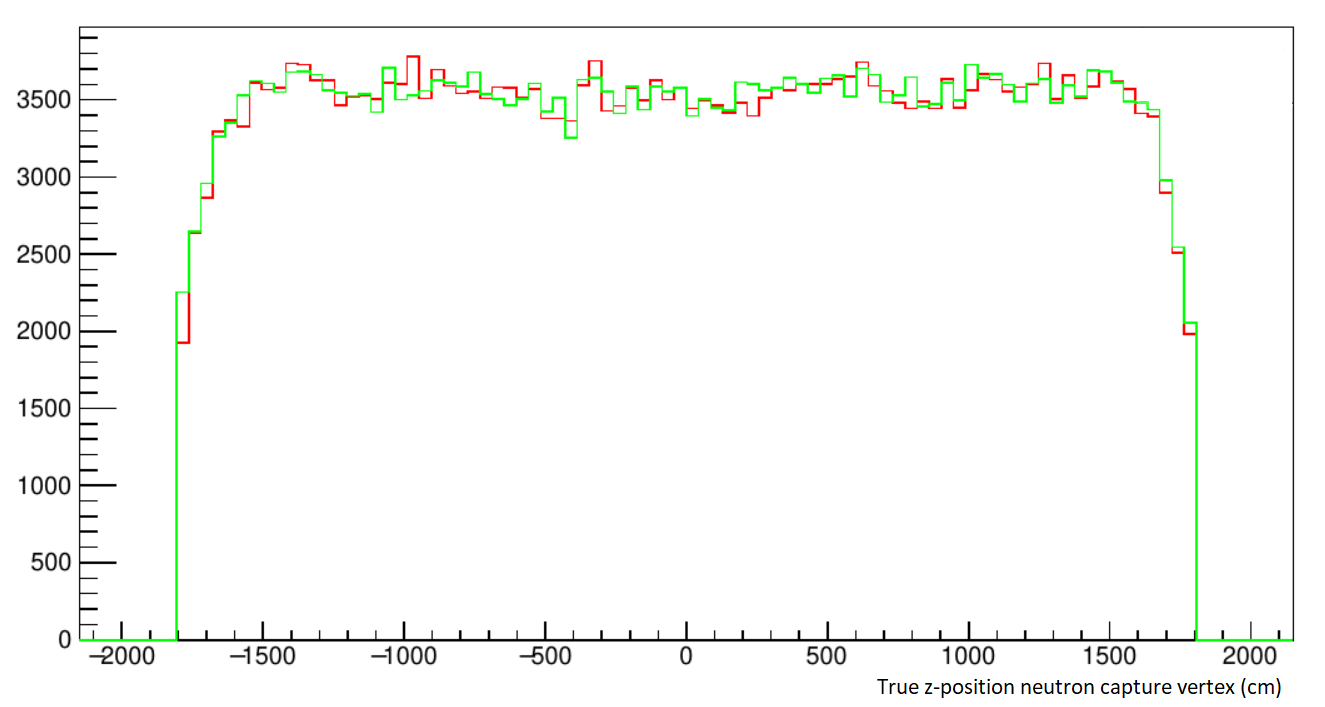
\includegraphics[width=0.5\linewidth]{Figures/zTrueCapturePos.png}}
    
    \caption{True neutron capture x-position (cm) (top left), true neutron capture y-position (cm) (top right) and true neutron capture z-position (cm)(bottom) }
    \label{fig:TrueNCapPos}
\end{figure}


    
\subsubsection{Truth information reduction cut plots}

After ensuring that the truth neutron tagging information was the same between the legacy and new NTag versions, the next step was to produce plots with the NCQE reduction cut criteria in order to see the distribution of neutrons for certain variables which satisfy the NCQE criteria. By rewriting aspects of the new NTag code to incorporate the BONSAI variables needed for the NCQE selection, the same reduction cut criteria could be applied to the new NTag code as it was to the legacy NTag code. Figure \ref{fig:TruCapTimeReduction} shows the number of true neutrons plotted against true neutron capture time for the legacy and new NTag, while Figure \ref{fig:TruCapNuNDistanceReduction} shows the number of true neutrons plotted against the distance between the true neutron and neutrino capture vertices for the legacy and new NTag.

\begin{figure}
    \centering
     \begin{subfigure}[b]{0.49\linewidth}
      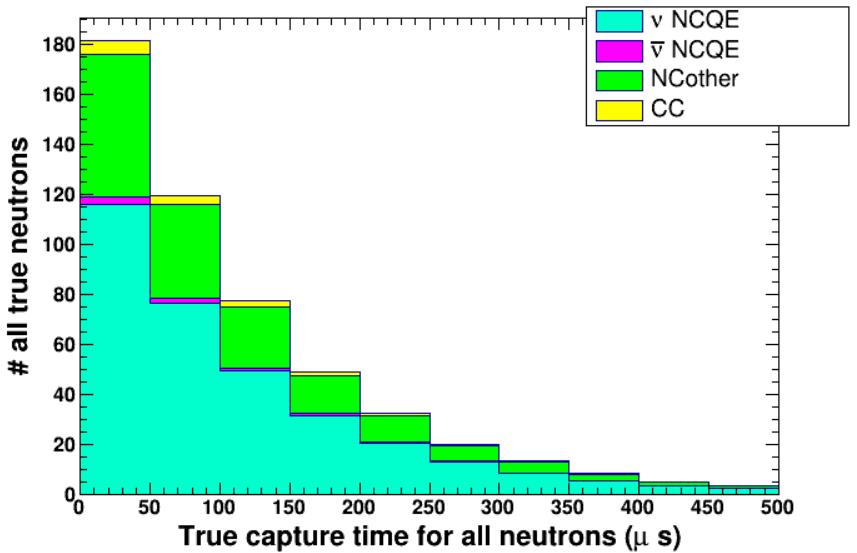
\includegraphics[width=\linewidth]{Figures/TrueCapTimeReductionLegacy.PNG}
     \end{subfigure}
     \begin{subfigure}[b]{0.49\linewidth}
       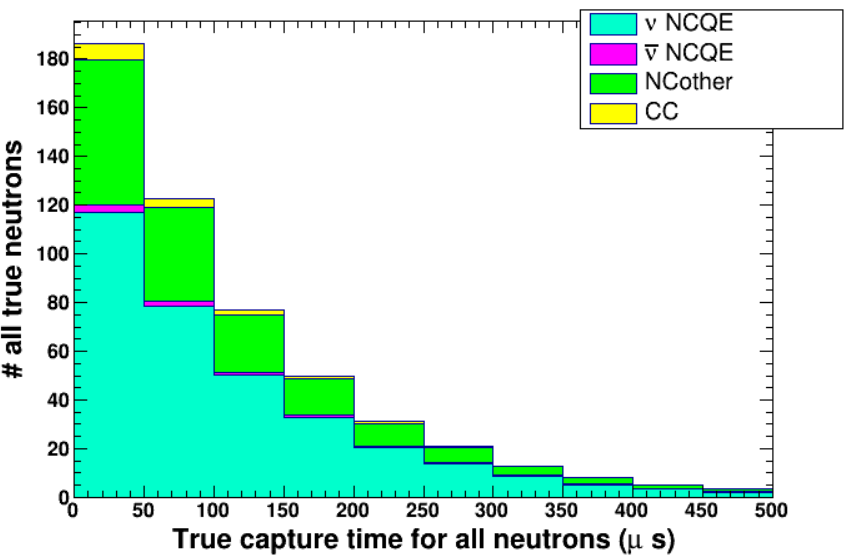
\includegraphics[width=\linewidth]{Figures/TrueCapTimeReductionNew.PNG}
      \end{subfigure}
      \caption{Number of true neutrons detected plotted against true neutron capture time for the legacy NTag (left) and the new NTag (right).}
      \label{fig:TruCapTimeReduction}
\end{figure}

\begin{figure}
    \centering
     \begin{subfigure}[b]{0.49\linewidth}
      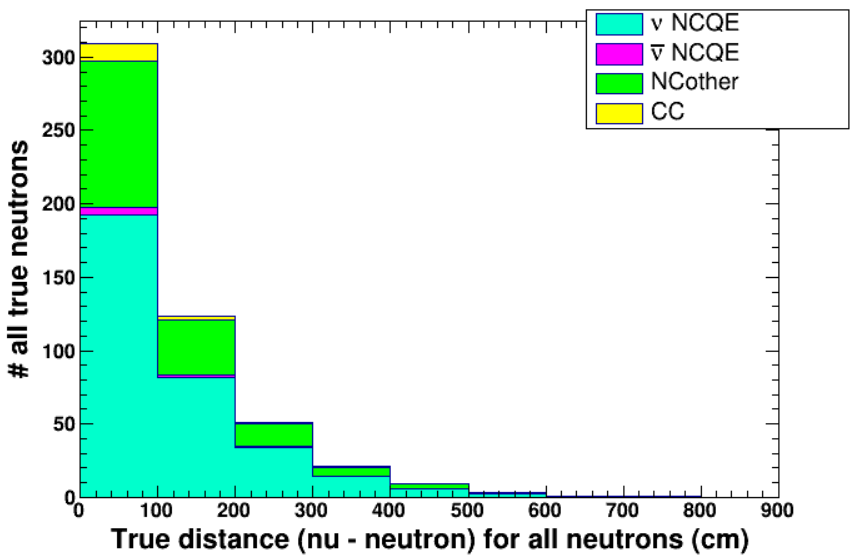
\includegraphics[width=\linewidth]{Figures/TruCapNuNDistanceReductionLegacy.png}
     \end{subfigure}
     \begin{subfigure}[b]{0.49\linewidth}
       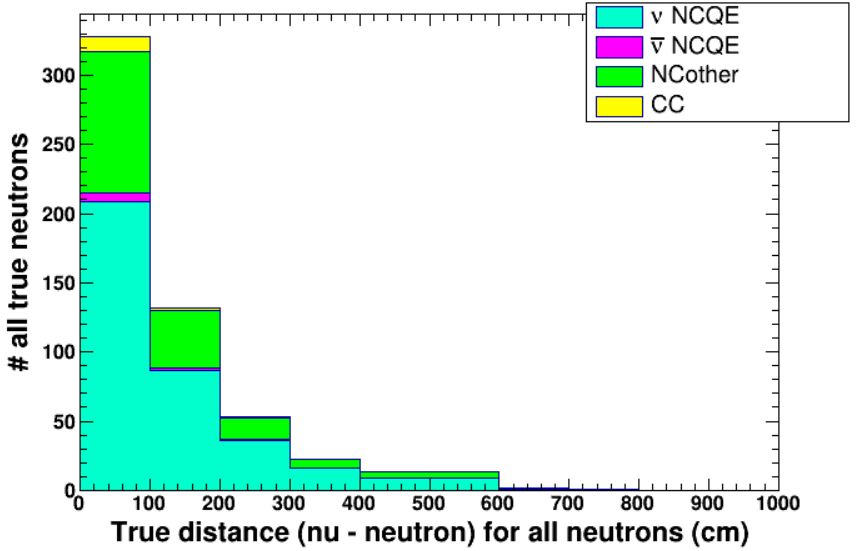
\includegraphics[width=\linewidth]{Figures/TruCapNuNDistanceReductionNew.png}
      \end{subfigure} 
      \caption{Number of true neutrons detected plotted against the distance between the neutrino and neutron capture vertices for the legacy NTag (left) and the new NTag (right).} 
      \label{fig:TruCapNuNDistanceReduction}
\end{figure}

With the level of $\mathrm{Gd}_{2}\left(\mathrm{SO}_{4}\right)_{3} \cdot 8 \mathrm{H}_{2} \mathrm{O}$ in the simulation being 0.026\%, the number of neutron captures on hydrogen and gadolinium should be approximately equal \cite{Sekiya_2020}. Figure \ref{fig:TruCapTimeReductionNewHGd} shows the the true capture time for the neutrons in the Monte Carlo seperated into captures on hydrogen and captures on gadolinium, and the distributions and the number of events look very similar, confirming this. Similarly, Figure \ref{fig:TruCapNuNDistanceReductionNewHGd} shows the distance between the neutrino interaction vertex and the true neutron capture vertex for captures on hydrogen and gadolinium. Once again the distributions are very similar, showing agreement with the equal number of captures.


\begin{figure}
    \centering
     \begin{subfigure}[b]{0.49\linewidth}
      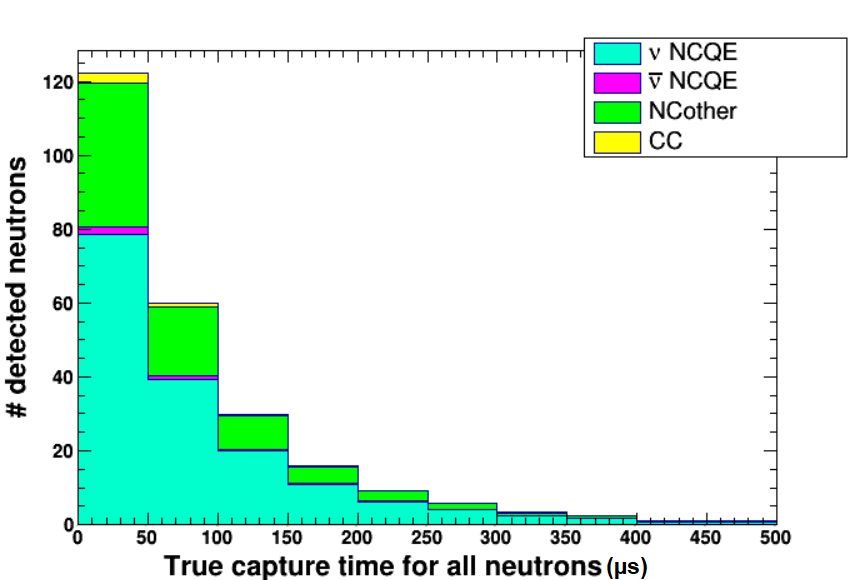
\includegraphics[width=\linewidth]{Figures/TruCapTimeReductionNewH.PNG}
     \end{subfigure}
     \begin{subfigure}[b]{0.49\linewidth}
       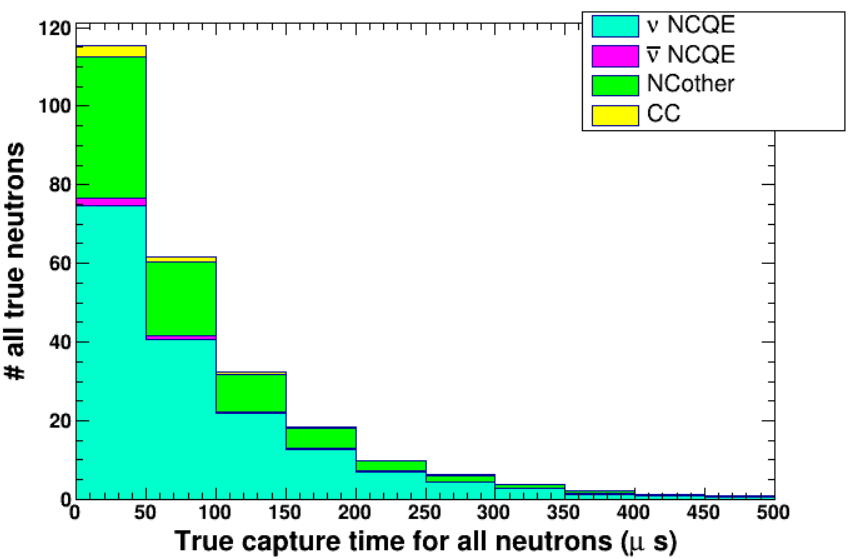
\includegraphics[width=\linewidth]{Figures/TruCapTimeReductionNewGd.PNG}
      \end{subfigure} 
      \caption{Number of true neutrons detected plotted against true neutron capture time for the new NTag, for captures on hydrogen (left) and gadolinium (right).}
      \label{fig:TruCapTimeReductionNewHGd} 
\end{figure}

\begin{figure}
    \centering
     \begin{subfigure}[b]{0.49\linewidth}
      \includegraphics[width=\linewidth]{Figures/TruCapNuNDistanceReductionNewH.PNG}
     \end{subfigure}
     \begin{subfigure}[b]{0.49\linewidth}
       \includegraphics[width=\linewidth]{Figures/TruCapNuNDistanceReductionNewGd.PNG}
      \end{subfigure} 
      \caption{Number of true neutrons detected plotted against the distance between the neutrino and neutron capture vertices for the new NTag, for captures on hydrogen (left) and gadolinium (right)}
      \label{fig:TruCapNuNDistanceReductionNewHGd} 
\end{figure}

\subsection{Primary selection criteria}

The rest of this Chapter focusses on analysis results from the new NTag algorithm, as this is what is currently being used by the collaboration. As input to searching for acceptable neutron candidates in the search window of 3 to 535 ns, the time of flight corrected PMT hit times is used. The reason for calculating the residual time of flight for the gamma hits is because the electrons produced from the Compton scattering of gamma rays produced by the neutron capture on hydrogen and gadolinium appear as a point-like source of Cherenkov radiation. Due to the differing optical path lengths that these photons have, there is a difference in PMT hit time. The difference in Cherenkov photon travel length before they hit different PMTs after the gamma rays from neutron capture Compton scatter off an electron needs to be taken into account via a time-of-flight (TOF) correction. Equation \ref{eq:TOF_correction} gives the equation for the residual hit times $t_{i}^{res}$, where $t_{i}$ is the hit time of the PMTs in the neutron search window and $TOF_{i}$ is given by Equation \ref{eq:TOF_calc}, where $PMT_{i}$ is the position vector of the hit PMT and $VTX_{\nu}$ is the position vector of the reconstructed neutrino vertex and $c_{wt}$ is the speed of light in the medium. The reason $VTX_{\nu}$ is used instead of the Compton scattering vertex is because this vertex is unknown. 

\begin{equation}
    t_i^{\text {res }} \quad=t_i-T O F_i \quad i \in\{\text { Hit PMTs }\}
    \label{eq:TOF_correction}
\end{equation}

\begin{equation}
T O F_i=\frac{\left\|\overrightarrow{P M T_i}-\overrightarrow{V T X_\nu}\right\|}{c_{w t}}
\label{eq:TOF_calc}
\end{equation}

Before the neutron candidate is passed to the secondary selection, other cuts are used to reject candidates which are not neutrons from NCQE interactions. Table \ref{table:new_selection_criteria} shows the three primary selection criteria. The first involves the width of the sliding window used for the neutron tagging search, which is set to 14 ns. The second is the hit tigger for the neutron candidate selection, which is set to 7 hits, which is the same for the previous NCQE Hydrogen-ntag analysis, with the maximum value of the hits set to 400. Third, the minimum time seperation between the gamma hits is set to 200 ns - the reason for this is to avoid double counting the same hit from the neutron capture candidate. 


\begin{table}
    $$
    \begin{array}{ccc}
    \hline \text{Criterion} & \text{Type} & \text{New} \\
    \hline \text { First } & \text{Timing window width} & 14 \mathrm{nsec} \\
    \text { Second } & \text{Hit trigger and max} & 7 \leq NH i t s \leq 400 \\
    \text { Third } & \text{Minimum hit seperation} & \Delta t_0 \geq 200 \mathrm{nsec}\\
    \hline
    \end{array}
    $$
    \caption{NTag primary selection criteria}
    \label{table:new_selection_criteria}
\end{table}

 One of the benefits of the addition of $\mathrm{Gd}_{2}\left(\mathrm{SO}_{4}\right)_{3} \cdot 8 \mathrm{H}_{2} \mathrm{O}$ is that the higher visible energy improves the neutron capture vertex resolution. Figure \ref{fig:vertex_resolution_ncap} shows the distance between the true and reconstructed neutron capture vertices for neutron capture in water Monte Carlo (taken from \cite{akutsu_thesis}) on the left, and from the Monte Carlo in this analysis on the right. It is clear that the resolution has improved, being reduced from 132.4 cm prior to the addition of gadolinium to 111.5 cm in this analysis.

 \begin{figure}
    \centering
     \begin{subfigure}[b]{0.49\linewidth}
      \includegraphics[width=\linewidth]{Figures/resolution_ncap_akutsu.PNG}
     \end{subfigure}
     \begin{subfigure}[b]{0.49\linewidth}
       \includegraphics[width=\linewidth]{Figures/resolution_ncap_hgd.png}
      \end{subfigure} 
      \caption{Distance between true and reconstructed neutron capture vertex in water Monte Carlo \cite{akutsu_thesis} (left) and from this analysis (right). The pink arrow on the left plot and the dashed blue line on the right plot shows the 68th percentile of the distributions.}
      \label{fig:vertex_resolution_ncap} 
\end{figure}


\subsection{Secondary selection criteria}
Due to the contamination of background events still present amongst the true neutron events after primary selection, a neural network (NN) is used to efficiently remove these background events, while trying to maximise the number of true neutron events. The output of the NN is used to indicate how likely a variable is to be signal/background candidate. Each of the candidates selected during the primary selection process has an associated reconstructed Compton scattering vertex calculated for it. In order to produce residual hit times that are less spread out than TOF-corrected hits towards the neutrino vertex, the TOF-corrected hits towards the Compton scattering vertex are used instead. The aim of searching for the Compton scattering vertex is to use a method by which the standard deviation of the residual times of the hits is minimised. Therefore the Compton scattering vertex $n_{VTX}$ is defined as in Equation \ref{eq:ncap_vtx}, where $r$ is a trial vertex and $t_i^{\text {res }}$ is the TOF-corrected hit time.

\begin{equation}
    n_{VTX}=\underset{r}{\operatorname{argmin}}\sqrt{\frac{1}{NHits} \sum_{i=1}^{NHits}\left[t_i^{\text {res }}(\vec{r})-\left\langle t^{\text {res }}(\vec{r})\right\rangle\right]^2}
\label{eq:ncap_vtx}
\end{equation}

 

By considering a set of trial vertices on a cubic grid and calculating the standard deviatiation of the residual hit times the minimisation process is performed. After this minimization cycle, a new cycle is performed on a finer and smaller grid and carries on until a certain level of precision is reached. 

When the Compton scattering vertex from neutron capture is found by this method, 12 variables which describe different aspects of the neutron candidate are calculated, using NTag. For each of the neutron candidates the vector of these variables are computed and fed into the neural network and this produces an output value which is between 0 and 1. These variables relate to different features regarding categorising hits from neutron capture on Gd or H, including the number of the hits from neutron capture, the isotropy of these hits, the Cherenkov angles of these hits and the position of the neutron vertex in the detector when capture occurs. The purpose of these variables is to tag the neutrons and better seperate tagged neutrons from accidentals and to distinguish when a capture occurs on hydrogen or gadolinium. A description of these variables are given below.


\underline{NTag variables}

The following twelve variables are fed into the TMVA neural network model for the secondary selection, and the TMVA reader and the input variables to get the classifier output:

\underline{NHits}

This is defined as the number of hits in a sliding timing window for the neutron candidate, however instead of this being set to a value of 10 nsec as it was for the neutron capture on hydrogen NCQE analyses, this was increased to 14 nsec in order to accomadate for the increased number of hits from gamma cascades from neutron capture on gadolinium.

\underline{N200}

This is the number of hits within -100 ns and +100 ns from the fitted time relative to the trigger. Signal events produce PMT hits which are close in time, while background events are more spread out, therefore alongside having the NHits variable, N200 is also used to create a wider timing window around the capture time of the candidate event. This spread of background events is clearly visible for the N200 variable both in Figure \ref{fig:pre_NN_signal} and Figure \ref{fig:post_NN_signal}: the distributions associated with neutron captures on hydrogen and gadolinium (red and green lines respectively) have distinct peaks, while the background events (magenta) have a more diffuse distribution. 

\underline{N1300}

This is the number of PMT hits in a 1300 ns timing window, specifically between -520 ns and +780 ns from the fitted time relative to the trigger. Similarly to N200 this is a much broader timing window than NHits.    

\underline{TRMS}

This calculates the standard deviation of the time-of-flight corrected PMT hit times from NHits. The spread of hit times varies between signal and background events, due to background events having a larger residual time spread than signal events: this is shown for the TRMS plot in Figure \ref{fig:pre_NN_signal}.

\underline{DWall}

DWall gives the difference from the fitted neutron vertex to the nearest wall in cm. This variable is used because the reconstructed vertex of background events are more likely to be near the inner detector wall, and therefore DWall can help distinguish background from signal events. 

\underline{DWallMeanDir}

This gives the distance from the fitted neutron vertex to the wall in the direction of the mean of the PMT hits for the neutron candidate in cm. The reason this variable is used alongside DWall is that there is also the aspect of the directionality of the hits to consider. Background hits do not have directionality due to them being a product of noise hits but signal events do have directionality due to these hits being produced by Compton scattered electrons originating from gammas produced by neutron capture. This is shown in the DWallMeanDir distribution in Figure \ref{fig:pre_NN_signal}, where the background events have a larger spread and also larger peak value than signal events.

\underline{OpeningAngleMean}
The next set of variables a related to the Cherenkov angle produced from a neutron candidate event: the first of these is OpeningAngleMean.
This calculates the mean of all possible opening angles calculated from 3 PMT hits from the neutron captures. Signal events which have PMT hits originating from Compton scattered electrons from 2.2 Mev gamma rays from neutron captures on hydrogen have Cherenkov opening angles which are centered around 42\degree, while neutron captures on gadolinium produce multiple gamma rays which would skew the value of OpeningAngleMean to be centered around higher values. This is reflected in Figure \ref{fig:pre_NN_signal}, where the background events have a slightly higher spread and therefore not such a strict angular depedence.

\underline{OpeningAngleStdev}

This is the standard deviation of all possible opening angles calculated from 3 PMT hits from the neutron captures. This variable emphasises what is seen in the OpeningAngleMean distribution, where background events have a larger spread than signal events, shown in Figure \ref{fig:pre_NN_signal} and Figure \ref{fig:post_NN_signal}. 

\underline{OpeningAngleSkew}

This is the skewness of all possible opening angles from 3 PMT hits from the neutron captures, calculated using

\begin{equation}
    \tilde{\mu}_3=\frac{\sum_i^N\left(X_i-\bar{X}\right)^3}{(N-1) * \sigma^{1.5}}
\end{equation}

where $X_{i}$ is the hit PMT, $\bar{X}$ is the mean of the 3-hit vector, N is the size of the vector of PMT hits, and $\sigma$ is the standard deviation of the PMT hits.

\underline{MeanDirAngleMean}

This variable takes the mean of angles between the direction of each hit from neutron capture and the mean of the direction of these hits. 

\underline{MeanDirAngleRMS}

This variable is simply the RMS of angles between each hit directon and mean hit direction.



\underline{$\beta_{l}$}

This variable is used because the signal and background events have a variation in the angular distribution of the hit PMTs. 
The $\beta_{l}$ variable defines the isotropy of the Cherenkov hits according to:

\begin{equation}
    \beta_{l}=\frac{2}{N_{H i t s}\left(N_{H i t s}-1\right)} \sum_{i \neq j} P_l\left(\cos \theta_{i j}\right)
\end{equation}

where $P_{l}$ are the Legendre polynomial's of order $l$ and $\theta_{ij}$ is the angle between hit PMTs relative to the neutron capture vertex. $\beta_{1}$, $\beta_{2}$, $\beta_{3}$,$\beta_{4}$, $\beta_{5}$ are all used as input variables to the NN in order to investigate the geometry of the neutron candidate hits related to spherical harmonics.

Figure \ref{fig:tagout} shows the neural network likelihood signal between 0 and 1 (TagOut), for all events, neutron capture on hydrogen candidates and neutron capture on gadolinium candidates. The blue arrow shows the cut on this variable (0.7), so that a neutron candidate that has been analysed is determined to be a signal neutron candidate if its value of TagOut > 0.7, and background if it is < 0.7. The value of 0.7 was chosen due to the amount of background events being sufficiently low enough past this value, while ensuring a substantial amount of neutron capture candidate signals on hydrogen and gadolinium.

\begin{figure}
    \centering
    \includegraphics[width=0.8\textwidth]{Figures/tagout.png}
    \caption{Neural network output signal likelihood }
    \label{fig:tagout}

\end{figure}


Seeing the signal from neutron captures on hydrogen and gadolinium pre and post neural network is also important along with the background events: these are shown in Figure \ref{fig:pre_NN_signal} and Figure \ref{fig:post_NN_signal}. 


\begin{landscape}
    \begin{figure}[t]
        \centering
        \hbox{\hspace{-0.5em}\includegraphics[width=\pdfpagewidth]{Figures/preNNvariablesbkg.PNG}}
        \caption{Number of events plotted against various neural network input variables prior to the neural network}
        \label{fig:pre_NN_signal}
    \end{figure}
\end{landscape}

\begin{landscape}
    \begin{figure}[t]
        \centering
        \hbox{\hspace{-0.5em}\includegraphics[width=\pdfpagewidth]{Figures/postNNvariablesbkg.PNG}}
        \caption{Number of events plotted against various neural network input variables after neural network output}
        \label{fig:post_NN_signal}
    \end{figure}
\end{landscape}



Figure \ref{fig:tagout} shows that the signal likelihood output is closer to 0 for far more neutron capture on hydrogen candidates than neutron capture on gadolinium candidates - this is also shown in Figure \ref{fig:pre_NN_signal} and Figure \ref{fig:post_NN_signal}, where the peaks for the neutron capture on hydrogen candidates are significantly more reduced in the post-NN plots than in the pre-NN plots, showing that noise events were more likely to be misidentified as neutron captures on hydrogen. These distributions also show that the value of NHits and also N200 for a neutron capture candidate is more likely to be greater for neutron candidates which are candidates on gadolinium than on hydrogen. Additionally, these plots also show that the opening Cherenkov angle related distributions were skewed towards greater values for gadolinium capture candidates than for hydrogen, due to the presence of the hits from the gamma cascade associated with neutron captures on gadolinium. 

After investigating the neutron candidates pre and post neural network to see the candidate signal distributions, it makes sense to evaluate how efficient the neutron tagging algorithm is. There are three stages at which the efficiency is calculated, pre-NN selection (i.e. seaching all the truth candidates prior to NN selection), after the NN classification (to show the efficiency of the classifier), and then the combination of these (the total tagging efficiency). Equation \ref{eq:efficiency_equations} shows how these three stages, $\varepsilon_{\text {Pre }}$, $\varepsilon_{\text {NN }}$ and $\varepsilon_{\text {NTag }}$ are defined.

\begin{equation}
\begin{aligned}
    & \varepsilon_{\text {Pre }}=\frac{\# \text { of truth candidates at pre }-\text { selection }}{\# of truth neutrons} \\
    & \varepsilon_{\mathrm{NN}}=\frac{\# \text { of tagged truth neutrons }}{\# \text { of truth candidates at pre-selection }} \\
    & \varepsilon_{\mathrm{NTag}}=\varepsilon_{\text {Pre }} \times \varepsilon_{\mathrm{NN}}=\frac{\# \text { of tagged truth neutrons }}{\# \text { of truth neutrons }}
\end{aligned}
\label{eq:efficiency_equations}
\end{equation}

The values of these efficiencies and their associated statistical uncertainties are shown in Table \ref{table:NTag_efficiency}, and are calculated seperately for captures on hydrogen and gadolinium and for both. 

\begin{table}
    $$
    \begin{array}{|l|l|}
    \hline & \text { Pre-selection efficiency } \\
    \hline \text { H + Gd } &50.0 \pm 0.10 \% \\
    \hline \text{ H } & 13.4 \pm 0.19 \% \\
    \hline \text { Gd } & 85.0 \pm 0.10 \% \\
    \hline & \text { NN classification efficiency } \\
    \hline \text { H + Gd } & 80.3 \pm 0.21 \% \\
    \hline \text { H } & 19.0 \pm 1.26 \% \\
    \hline \text { Gd } & 89.6 \pm 0.26 \% \\
    \hline & \text { Total efficiency } \\
    \hline \text { H + Gd } & 40.2 \pm 0.21 \% \\
    \hline \text { H } & 2.5 \pm 0.16 \% \\
    \hline \text { Gd } & 76.2 \pm 0.20 \% \\
    \hline
    \end{array}
    $$
    \caption{NTag pre-selection, NN classification and total efficiencies}
    \label{table:NTag_efficiency}
\end{table}

These efficiencies are as expected, with the efficiency of neutrons captured on gadolinium being much greater than that of captures on hydrogen, due to the gamma cascade making it better able to be differentiated than from the 2.2 MeV from the neutron capture on hydrogen. However, as the errors on the efficiency in Table \ref{table:NTag_efficiency} are purely statistical (i.e.produced from the number of neutrons in the MC), it is beneficial to do a comparison with an efficiency measurement from actual neutron capture data. In order to assess the validity of the efficiencies from the Monte Carlo, a comparison of the efficiency with data taken from an Am/Be neutron source is used. As mentioned in Chapter 3, the Am/Be source produces a prompt 4.4 MeV gamma ray along with a neutron, with the same prompt and delay signal pattern as NCQE interactions, and similarly to the MC, a timing distribution of hits relative to the 4.4 MeV trigger can be produced for the Am/Be data. As shown in Figure \ref{fig:efficiency_dwall}, the efficiency of the neutron capture changes relative to the DWall cut value, and as a result it was advisable to check the efficiency of neutron capture using Am/Be data at different positions in the detector. Table \ref{table:ambe_positions} shows the runs and positions (x,y,z) of Am/Be data used in this analysis.

\begin{figure}
    \centering
    \includegraphics[width=0.8\textwidth]{Figures/efficiency_dwall.png}
    \caption{Neural network output signal likelihood }
    \label{fig:efficiency_dwall}

\end{figure}


\begin{table}
    $$
    \begin{array}{|l|l|l|l|l|}
    \hline \text{Run} & \text {Data taking time } & \text{Position (m)} \\
    \hline 85622 & \text { 1 hour} & \text{(0,0,0)} \\
    \hline 85617 & \text { 30 min} & \text{(0,0,+12)} \\
    \hline 85586 & \text { 30 min} & \text{(-12,0,0)} \\
    \hline
    \end{array}
    $$
    \caption{Am/Be data run numbers, data taking time and Am/Be source positions}
    \label{table:ambe_positions}
\end{table}

First, comparison was done between the MC and the Am/Be data from Run 85622, the 1 hour measurement taken in the central (0,0,0) source position, by looking at the timing distribution from the 4.4 MeV trigger signal. The following event cuts were used in order to select neutron capture events using this data: the total event charge deposit for the inner detector PMTs to be between 850 and 1150 photoelectrons, the time difference from the previous event should be greater than 1 millisecond, and the number of outer detector PMT hits should be less than 10. In order to find the efficiency of the neutron captures with this Am/Be data, an exponential fit was made to the timing distribution, and this is shown in Figure \ref{fig:ambe_centre}. Similar plots were made for the Am/Be source data taken for the (0,0,+12 m) and (-12 m,0,0) positions.


\begin{figure}
    \centering
    \includegraphics[width=0.8\textwidth]{Figures/ambe_centre.png}
    \caption{Fitted time relative to the trigger signal with exponential fit (red) for the Am/Be data taken in the centre position (0,0,0)}
    \label{fig:ambe_centre}
\end{figure}

\begin{figure}
    \centering
    \includegraphics[width=0.8\textwidth]{Figures/ambe_data_+12z.png}
    \caption{Fitted time relative to the trigger signal with exponential fit (red) for the Am/Be data taken at (0,0,+12 )}
    \label{fig:ambe_+12z}
\end{figure}

\begin{figure}
    \centering
    \includegraphics[width=0.8\textwidth]{Figures/ambe_data_-12x.png}
    \caption{Fitted time relative to the trigger signal with exponential fit (red) for the Am/Be data taken at (-12,0,0).}
    \label{fig:ambe_-12}
\end{figure}

Table \ref{table:ambe_tau_chi2} shows the value of tau for each of these positions, along with the $\chi^{2}$/ndf value for the exponential fit and the value of the neutron capture efficiency calculated from the Am/Be data at each of these positions. Equation \ref{eq:efficiency_ambe_calculation} shows the method by which the efficiency for the neutron capture on Am/Be data is calculated, where $N$ is the number of neutron captures, $B$ is the fitted constant background value, and NTag TMAX and NTag TMIN are the end and start times of the neutron tagging algorithm.  





\begin{equation}
    \text { Efficiency }=\frac{(\text {N } - (\text{B} \cdot \text {no. of bins }  \cdot (\text{NTag TMAX - NTag TMIN}) / (\text{fit time range})))  }{\text { no. of events }}
    \label{eq:efficiency_ambe_calculation}
\end{equation}

\begin{table}
    $$
    \begin{array}{|l|l|l|l|l|}
    \hline \text{Position (m)} & \text {Time constant (tau) value ($\mu$ s) } & \text{$\chi^{2}$/ndf} & \text{Efficiency (\%)} \\
    \hline \text{Centre (0,0,0)} & 114.8 \pm 2.5  & 1.01 & 40.7 \\
    \hline \text{(0,0,+12 )} & 118 \pm 3.5 & 1.27 & 39.4 \\
    \hline \text{(-12,0,0)} & 110 \pm 3.7 & 1.17 & 40.7 \\
    \hline
    \end{array}
    $$
    \caption{Am/Be time constant value and $\chi^{2}$/ndf value of exponential fit}
    \label{table:ambe_tau_chi2}
\end{table}

This level of variation for the time constant is within normal limits, especially considering the associated errors, and the $\chi^{2}$/ndf values for each shows that the exponential fit to the data is good. Figure \ref{fig:MC_time_constant} shows the equivalent fitted time from the prompt event for the NCQE MC, which has a corresponding time constant value of 115.6 $\pm$ 0.8 $\mu$ s, and a neutron tagging efficiency, as shown in Table \ref{table:NTag_efficiency} of 40.2\%: these values are in good agreement with the values shown in Table \ref{table:ambe_tau_chi2}. 

\begin{figure}
    \centering
    \includegraphics[width=0.8\textwidth]{Figures/MC_fitT.png}
    \caption{Fitted time relative to the trigger signal with exponential fit (red) for the NCQE MC}
    \label{fig:MC_time_constant}
\end{figure}

